% !TeX program = pdflatex
% !TeX spellcheck = es_ES

\documentclass{article}
\usepackage[utf8]{inputenc}
\usepackage[spanish,mexico]{babel}

\usepackage[a4paper,top=3cm,margin=4cm,bottom=5cm]{geometry}
\usepackage[symbol]{footmisc}
\renewcommand*{\thefootnote}{\fnsymbol{footnote}}
\usepackage{fancyhdr}
\setlength{\headheight}{15.2pt}
\pagestyle{fancy}
\lhead{\href{http://whittileaks.com}{\sf whittileaks.com} }
%\chead{Metalurgia Fisica -- 2ndo Parcial}

\usepackage{graphicx}
%% FOOTNOTES

%% 
\usepackage{enumitem}
\title{Metallurgy}
\author{Patricio Whittingslow}
\date{June 2019}
\newcommand{\Bs}{B\ensuremath{_{1}}}
\newcommand{\Aone}{A\ensuremath{_{1}}}
\newcommand{\Atwo}{A\ensuremath{_{2}}}
\newcommand{\Athree}{A\ensuremath{_{3}}}
\newcommand{\HB}{\ensuremath{\mathrm{HB}}}
\newcommand{\HRC}{\ensuremath{\mathrm{HRC}}}
\newcommand{\Tdf}{\ensuremath{T_{\mathrm{df}}}}
\newcommand{\Acm}{A\ensuremath{_{\mathrm{cm}}}}
\newcommand{\grad}{\ensuremath{^\circ \mathrm{C}}}
\newcommand{\cementita}{\ensuremath{\mathrm{Fe}_3 \mathrm{C}}}
\usepackage{soulutf8}
\usepackage{siunitx}
\usepackage{multirow}
\usepackage{caption,subcaption}
\usepackage{hyperref}
\hypersetup{
    colorlinks,
    citecolor=black,
    filecolor=black,
    linkcolor=black,
    urlcolor=black
}

\usepackage{natbib}
\bibliographystyle{plainnat}

\newcommand{\um}{\si{\micro \meter}}
\newcommand{\goright}{\ensuremath{\rightarrow}}


% \cfoot{\thepage}
% PLOTTING
\usepackage{pgfplots}

\begin{document}


\maketitle

\tableofcontents

\part{Introducción a la Metalurgia}


\section{Diferencia entre lo micro y macro}

Los conjuntos diseñados por ingenieros tienen una forma \textbf{geométrica} y un \textbf{material}. Ambas son propiedades macroscópicas. 

Sin embargo, lo que determina en gran parte las propiedades de una pieza es su \textbf{estructura} al nivel atómico (Å) y microscópico (micrómetros). Estas no son evidentes al ojo humano y se necesita de instrumentos y técnicas para poder detectar y caracterizar estas estructuras.

Un objetivo fundamental de la metalurgia física es tratar de relacionar los aspectos macroscópicos perceptibles con los aspectos microscópicos y submicroscópicos mediante métodos \textbf{netamente científicos}. La metalurgia física es una ciencia aplicada.

\section{Nociones de materiales}

\subsection{Grupos de Materiales}

\begin{description}
    \item[Metales] Materiales con enlaces metálicos
    \item[Polímeros] Sustancias inorgánicas con enlaces no metálicos
    \item[Polímeros] Matríz metálica, polimérica o cerámica con partículas o fibras poliméricas o cerámicas 
\end{description}


\subsection{Características de los metales}
Como clase de material, los metales son aquellos materiales cuyos átomos están unidos mediante un enlace metálico. Algunos materiales poseen enlaces no metálicos y son considerados metales porque su enlace metálico es el que prevalece, como es el caso para la mayoría de los metales estudiados.

\begin{itemize}
    \item Deformables plásticamente
    \item Fáciles de conformar y unir
    \item Alta tenacidad
    \item Alta resistencia mecánica
    \item Alta rigidez
    \item Bajo costo
    \item Alta conductividad eléctrica y térmica
    \item Fácilmente reciclables
    \item Baja resistencia a la corrosión
    \item Alta densidad
\end{itemize}



\subsection{Aleaciones metálicas}

Se define como un material compuesto por varias clases de átomos (metálicos y/o no metálicos) unidos mediante un enlace principalmente metálico.

El \textbf{elemento base} de la aleación es el elemento químico mayoritario y siempre es de carácter metálico. Los \textbf{aleantes} son elementos cuya presencia se debe a una adición \textit{intencional} durante el proceso de fabricación de la aleación. Cumplen funciones específicas. En general hay un \textbf{aleante principal} que le otorga las características principales a la aleación y no tiene porque ser el de mayor proporción.

Los átomos que no fueron agregados intencionalmente sino que provienen de alguna/s de las materias primas usadas para la fabricación de la aleación (mineral, fundente, combustible, oxidante) y no han podido ser totalmente eliminados en el proceso de fabricación se llaman \textbf{residuales}. Se pueden categorizar en dos clases

\begin{description}
    \item[Residuales no nocivos] No tienen efectos negativos de importancia y pueden hasta mejorar alguna propiedad
    \item[Residuales nocivos o impurezas] Influyen negativamente en algunas propiedades de importancia para la aleación. Su reducción conlleva con un aumento del costo.  
\end{description}

\section{Unión entre átomos}

\begin{figure}
    \centering
    \begin{tikzpicture}[>=stealth]
    \begin{axis}[
        xmin=-.1,xmax=4,
        ymin=-2,ymax=3,
        axis x line=middle,
        axis y line=middle,
        axis line style=<->,
        xlabel={$d$},
        ylabel={$U$},
        cycle list name=exotic,no marks
        ]
        \addplot expression[domain=.2:3.7,samples=100]{1/x} 
                    node[pos=0.5,anchor=south west]{Atracción electrostática}; 
        \addplot expression[domain=.4:3.7,samples=80]{(x-2*(x+.04)^2)/((x+.04)^4)}  
        node[pos=.7,anchor=north west]{Energía de la unión};
        \addplot expression[domain=.2:3.7,samples=80]{-(x-1.6*x^2)/((x)^4)}  
        node[pos=.96,anchor=south west]{Fuerza neta de la unión};
        \addplot expression[domain=.5:3.7,samples=80]{-1/(x+.3)^5}  node[pos=.3,anchor=north west]{Repulsión de muy corto alcance};
    \end{axis}
\end{tikzpicture}
\caption{Fuerzas que intervienen en una unión iónica. El punto donde la fuerza neta cruza el eje $x$ se denomina la distancia de equilibrio $d_0$ y es la distancia nominal entre átomos en un material. Este punto coincide con el mínimo de energía de la unión.}
\end{figure}

\begin{itemize}
    \item El mínimo de energía ($U_0$) está relacionado con la temperatura de sublimación y fusión
    \item La pendiente de la curva de la fuerza neta sobre $d_0$ son proporcionales al módulo elástico del metal (se relaciona también con la curvatura de la energía sobre $d_0$ también)
    \item La asimetría de la curva de energía está relacionada con el coeficiente de dilatación del metal. Cuanto más empinada cerca de 0 y más chata alejándose de cero, más se dilata el material.
\end{itemize}



Al \textbf{aumentar} la energía de la unión, la distancia de equilibrio ($d_0$) disminuye (\textbf{disminuyendo la curvatura de la energía}), la curva de energía se vuelve \textbf{más simétrica}. En consecuencia puede decirse que, en términos generales, en los metales puros se cumple que a mayor punto de fusión es \textit{mayor} el módulo elástico y \textit{menor} el coeficiente de dilatación lineal.

\section{Estructura cristalina de metales}

En estado sólido los metales son cristalinos, es decir que los átomos ocupan posiciones ordenadas dentro de una estructura. Existen materiales metálicos sin ordenamiento en su estructura.

Existen materiales metálicos sin ordenamiento en su estructura (vidrios metálicos), pero son la excepción.

\begin{description}
    \item[Red cristalina] Red de puntos imaginarios que ocupan posiciones ordenadas en el espacio de modo que cada punto tiene idénticos alrededores
    \item[Motivo] Conjunto de átomos con una configuración determinada. Ocupa cada nodo de la red.
    \item[Estructura cristalina]  Red ordenada de puntos ubicándose en cada uno de ellos un mismo motivo constituido por átomos de metal
    \item[Parámetro de red] es la distancia entre átomos medida en las direcciones de los ejes principales de la celda de la red. Dependiendo de la configuración de la red (FCC/HCP/BCC) puede haber más de un parámetro. Suele ser del orden de unas décimas de nanómetro para metales.
\end{description}

\subsection{Características de estructuras cristalinas en metales}

\subsubsection{Estructura FCC}
Es una de las dos estructuras de máxima compacidad.
En general los FCC son metales de alta ductilidad y maleabilidad, baja tensión de fluencia, y alta tenacidad que además no presentan transición dúctil-frágil. 

\subsubsection{Estructura HCP}
Es una de las dos estructuras de máxima compacidad. Los HCP en general son metales menos dúctiles y más anisotrópicos que los FCC o BCC.


\subsubsection{Estructura BCC}
No posee planos de máxima compacidad. Los BCC poseen menor ductilidad y tenacidad que los FCC pero mayor tensión de fluencia. Presentan transición dúctil-frágil.

\subsection{Índices de Miller (incompleto)}

\subsection{Defectos cristalinos}






% !TeX spellcheck = es_ES
% !TeX root = ../metalurgy.tex
\part{Curvas de transformación tiempo-temperatura (TTT) y CCT}
Tambien conocidos como diagramas de transformación isotérmica, son tres aspectos los que dominan estas curvas:
\begin{itemize}
    \item Tiempo: Una vez que la temperatura de la austenita baja por debajo de \Aone se vuelve inestable y comienza a transformarse con el tiempo. 
    \item Morfología: Distribución, tamaño y forma de los productos obtenidos a partir de su transformación. son clave para las propiedades que se obtienen.
    \item Fases que no están en equilibrio: La aparición de fases fuera de equilibrio, como por ejemplo, la martensita
\end{itemize}
Los CCT son \textit{Continuous Cooling transformation} para enfriamiento a $\frac{\partial T}{\partial t}= \text{constante}$.


\begin{figure}[ht]
    \centering
    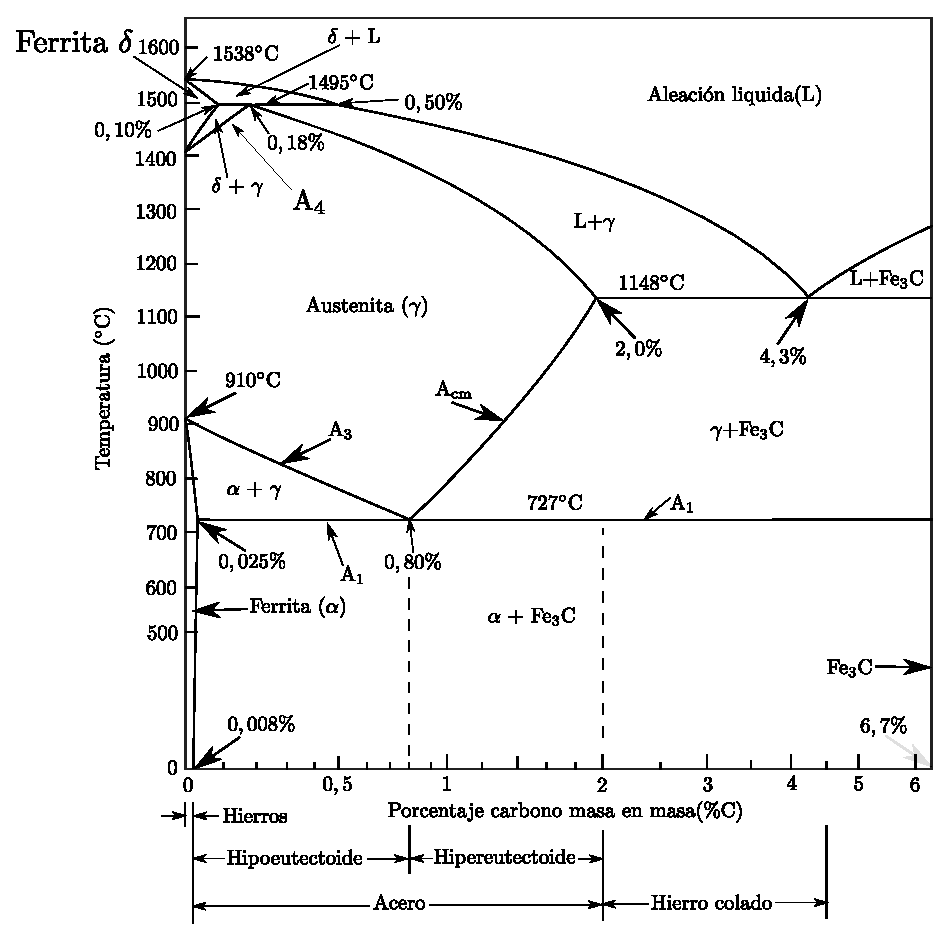
\includegraphics[width=1\textwidth]{fig/diagAceroreal.eps}
    \caption{Diagramas de fases para aceros.}
    \label{fig:diagAceros}
\end{figure}

Fases
\begin{itemize}
    \item Perlita: Morfología laminar, su transformación se favorece con mayor coeficiente de difusión.
    \item Bainita: Morfología con $\alpha$ en listones y carburos discretos
    \item Martensita: Misma composición que austenita pero red cristalina diferente (BCT) y distorsionada. Contiene zonas de austenita.
\end{itemize}



\section{Acero eutectoide}
Se comienza estudiando las transformaciones isotérmicas de la austenita
\begin{figure}[htb!]
    \centering
    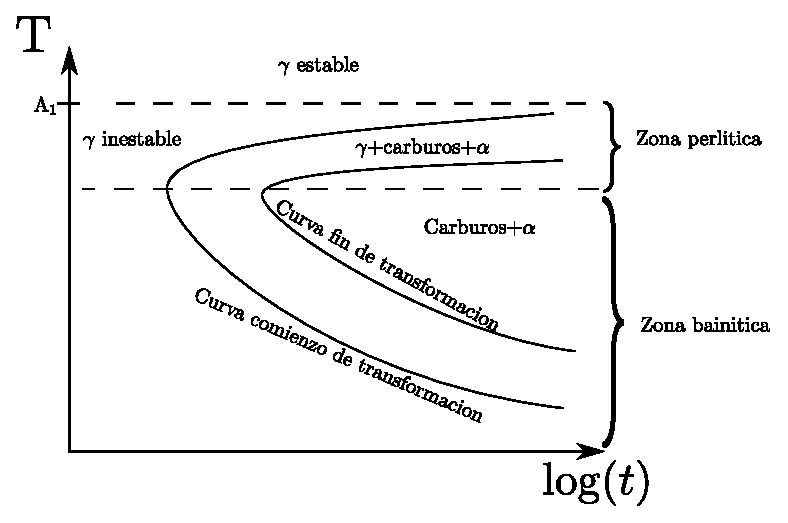
\includegraphics[width=\textwidth]{fig/TTTbasic.eps}
    \caption{Diagrama para transformación isotérmica de la austenita para un acero \textbf{eutectoide}.}
    \label{fig:diagTTTbasico}
\end{figure}

\begin{figure}[htb!]
    \centering
    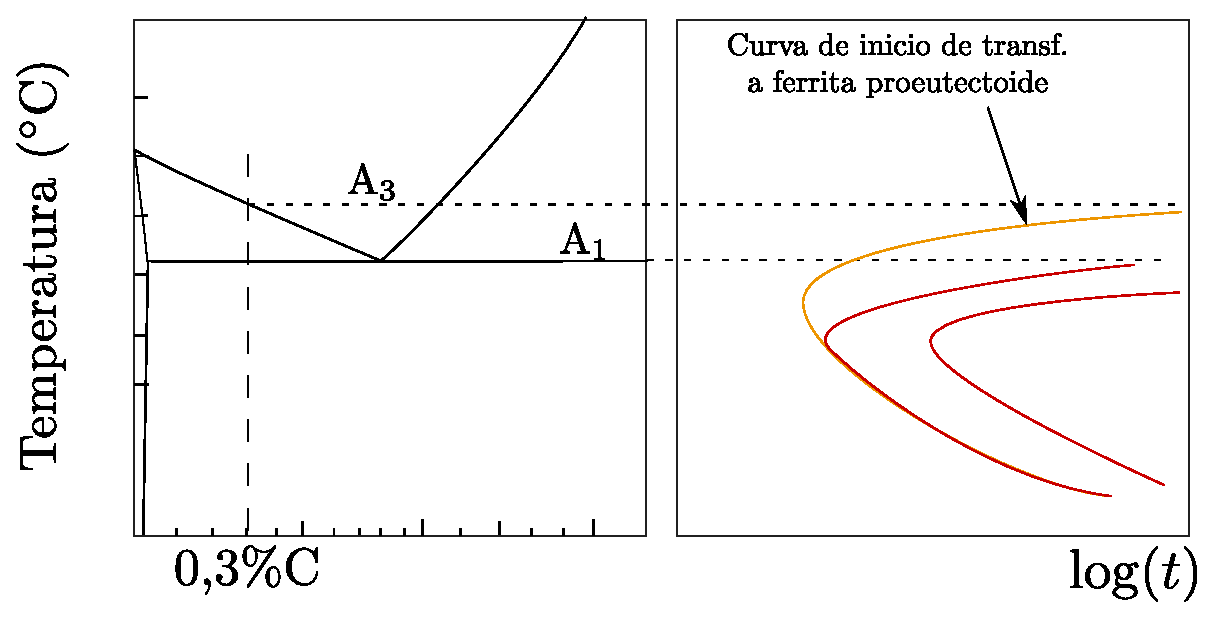
\includegraphics[width=\textwidth]{fig/diagTTThipo.eps}
    \caption{Diagrama para transformación isotérmica de la austenita para un acero \textbf{hipoeutectoide} (0,3\%).}
    \label{fig:diagTTThipo}
\end{figure}

\begin{figure}[htb!]
    \centering
    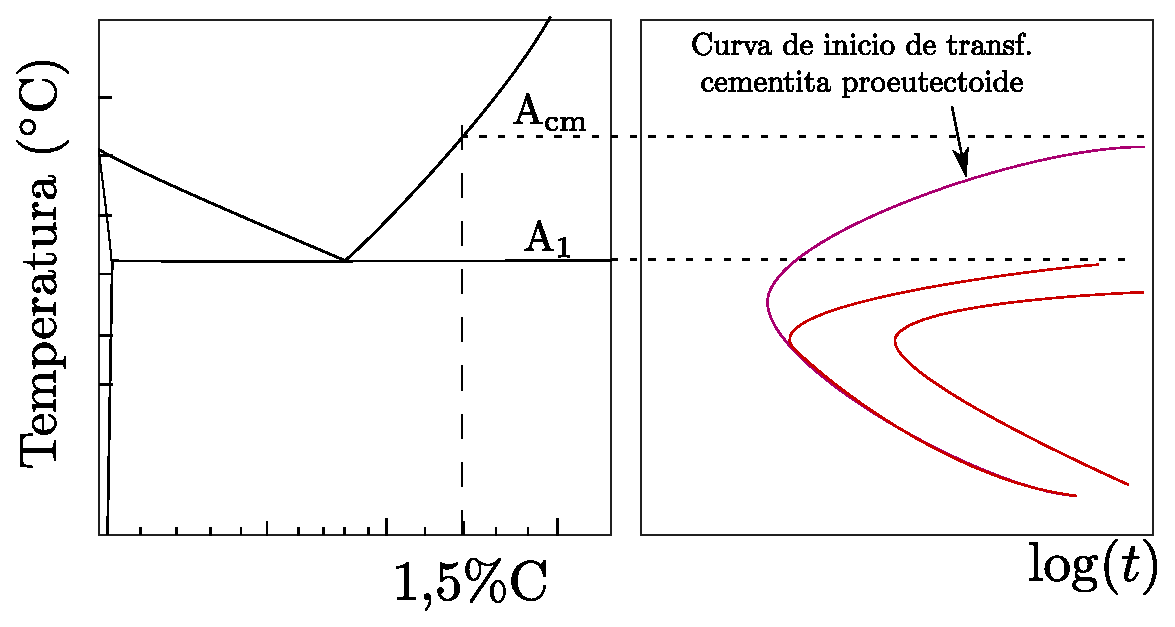
\includegraphics[width=\textwidth]{fig/diagTTThiper.eps}
    \caption{Diagrama para transformación isotérmica de la austenita para un acero \textbf{hipereutectoide} (1,5\%).}
    \label{fig:diagTTThiper}
\end{figure}

La nariz de la figura \ref{fig:diagTTTbasico} se da porque hay competencia entre la \textbf{fuerza impulsora} $\Delta G$ (dominante a bajas temperaturas) y el \textbf{coeficiente de difusión de carbono} $D_c$ (aumenta con temperatura).

Transformación perlítica



\section{Competencia entre G y D}
A temperaturas cercanas a \Aone la difusión domina mientras que a bajas temperaturas hay alta fuerza impulsora debido a que la inestabilidad de la austenita. Hay una temperatura a la cual se complementan y la transformación tiene una velocidad máxima, en la figura \ref{fig:diagTTTbasico} seria la nariz (450 a 600 \grad).

\section{Microconstituyentes}
Los productos de transformación de la austenita que combinan
ferrita y carburos de Fe, así como las fases proeutectoides, se denominan genéricamente \textbf{microconstituyentes} para diferenciarlos de las verdaderas fases que los componen.
\begin{itemize}
    \item Si enfriamos justo por debajo de \Aone~ la fuerza impulsora va ser baja  y van a prevalecer los sitios de nucleacion preferencial (bordes de grano). Comienza a nuclear a la par la ferrita y la cementita cooperativamente formando un microconstituyente con morfologia laminar denominado \textbf{perlita}. Ocurre por arriba de la nariz para subenfriamientos bajos ($<170\grad$).
    \item En cambio, en el rango de temperaturas por debajo de la nariz la ferrita nuclea primero, adopta una morfología de listones, y los carburos ya no son laminares sino discretos con forma de placas más o menos cortas. Por otra parte la transformación en esta zona tiene un mecanismo diferente al aquel que ocurre a altas temperaturas. Los microconstituyentes obtenidos en esta zona se denominan genéricamente \textbf{bainitas} y los hay de varios tipos.
    \item Finalmente, a temperaturas muy bajas ($<$ 350\grad) la austenita subenfriada transforma anisotérmicamente y sin difusión a una fase metaestable denominada martensita.
\end{itemize}


\section{Perlita}
Para generar perlita se requiere un alto coeficiente de difusión de carbono ya que se están generando zonas de muy bajo carbono (ferrita $\alpha$) y zonas de alto carbono (cementita $\cementita$) lo que requiere mucha difusión partiendo de austenita ($\gamma$). Prevalecen los sitios de nucleación preferencial debido a la baja fuerza impulsora $\Delta G$.

El \textbf{espaciado interlaminar} $S$ es el principal parámetro geométrico de la perlita. Tiene gran importancia y determina muchas propiedades. Es la distancia entre laminas contiguas de la misma fase medida perpendicularmente al eje longitudinal de las laminas (básicamente miras la foto de microscopio de electrones y ves cuanto espacio hay entre comienzos de dos laminas de cementita/ferrita). Existe la perlita gruesa ($S\approx 1\si{\micro \meter}$) y perlita fina $S< 0,3\si{\micro \meter}$. A mayor subenfriado menor es $D_c$, menos se puede desplazar el carbono y por ende menor va ser la distancia entre laminas de \cementita~ y $\alpha$.
\begin{equation}\label{eq:StoPerliteStrength}
    R_{p 0,2}, R_{m}, H V \propto S^{-\frac{1}{2}}
\end{equation}

Perlita mas fina trae dureza, resistencia y mayor tensión de fluencia. A su vez es mas difícil de formar, mecanizar etc.

\section{Transformación Martensita}
Cuando la austenita se sobrenfría hasta temperaturas muy bajas se produce una transformación sin difusión de C donde, en un volumen discreto de material, los átomos de Fe experimentan un movimiento cooperativo, pequeño, y casi simultáneo. Esto da por resultado una fase metaestable de igual composición química que la austenita que le dio origen pero con una estructura cristalina diferente. Esta fase se denomina martensita y la transformación se llama transformación martensítica.

En los aceros al C y de baja aleación la martensita tiene estructura tetragonal centrada en el cuerpo (\textit{Body Centered Tetragonal}, BCT). El C, al no poder difundir distorsiona la red y hace que en cambio de nuclearse la fase estable BCC aparezca una fase metaestable BCT.

El movimiento cooperativo genera tensión y deformación en la fase madre. Esta deformación puede causar fisuras y agravar el fenómeno de la fatiga. No hay difusión en la transformación martensítica y se dice que es atérmica (o anisotérmica), es decir que no evoluciona isotérmicamente sino que la fracción de martensita crece en tanto se siga subenfriando la austenita remanente.

$M_s$ es la temperatura de inicio de la transformación martensítica. $M_f,M_{90}$ en principio es la temperatura a la que finaliza dicha transformación. Siempre queda una fracción de austenita muy resistente a la transformación y por ende nunca se puede realmente medir la temperatura de transformación total $M_f$.\footnote{En realidad se define $M_f$ como el límite de 99\% transformación martensítica (definida como fracción de volumen), la temperatura a la cual toda la austenita se convierte a martensita es sustancialmente menor a $M_f$ \cite{gottstein2013physical}.} El subíndice indica la fracción (sobre cien) de martensita producida.

$M_s$ y $M_f$ dependen fuertemente de la composición química de la austenita, con excepción del Cobalto.
\begin{equation}
    M_s=539-423\cdot \% \mathrm{C}-30,4\cdot \% \mathrm{M n}-12,1\cdot \% \mathrm{Cr}-17,7\cdot \% \mathrm{Ni}-7,5\cdot \% \mathrm{Mo}
\end{equation}
como se ve en la ecuación arriba, componentes químicos hacen bajar la temperatura del comienzo de la transformación de austenita. El nitrógeno también tiene un efecto similar al carbono. $M_f$ también baja con aumento de aleantes.

\subsection[Temperatura {\it Md}]{Temperatura $M_d$}
Por debajo de cierta temperatura denominada ($M_d> M_s$), la
deformación plástica aplicada a la austenita provoca la transformación a martensita. El porcentaje de martensita aumenta al aumentar la cantidad de deformación plástica aplicada a la austenita a una determinada temperatura, y al disminuir la temperatura a la cual se aplica la deformación. $M_d$ también depende de la composición química de la austenita y baja al aumentar la cantidad de elementos disueltos en dicha fase. Esta característica cobra gran importancia práctica en el caso de los aceros inoxidables austeníticos. 

\subsection{Estructura Martensítica}
En realidad la estructura BCT de la martensita es una red BCC distorsionada por causa de la presencia del carbono en solución solida sobresaturada. Durante la transformación un eje (denominado \textbf{c}) se achica y otro eje (\textbf{a}) se ensancha, generando una expansión neta dependiente del carbono \footnote{La relación $c/a$ incrementa con la concentración de carbono \cite{gottstein2013physical}.}
\[
\varepsilon_{\Delta V \%} = 4,64-0,54\cdot (\% \mathrm{C})
\]



En martensitas de ``bajo'' carbono (menor a 0,6\%) se presentan los cristales en forma de listones paralelos de ancho 0,2 a 0,5\um~  formando paquetes entre ellos. Esta estructura contiene una gran cantidad de dislocaciones ($10^{11}$ disl/cm$^2$).

En martensitas de ``alto'' carbono (mayor a 0,8\%) y $M_s$ es lo suficientemente baja los cristales adoptan forma lenticular sin formación de paquetes. El plano de habito de estas estructuras puede ser el $\{225 \}_\gamma$ o el $\{259 \}_\gamma$ dependiendo del porcentaje de carbono. Debido a esto se pueden tener dos placas adyacentes con planos diferentes dándole un aspecto caótico a la estructura y generando microfisuras.

La dureza de la martensita se debe a los siguientes factores
\begin{itemize}
    \item \hl{Endurecimiento por solución solida: intersticial del carbono}
    \item \hl{Interacción dislocaciones - carbono segregado. Una vez cristalizada la martensita el carbono se puede segregar a sitios donde baja la energía del sistema. Las dislocaciones son lugares preferenciales (anclaje = dureza agregada)}
    \item Interacción entre dislocaciones
    \item Gran cantidad de bordes de grano (bajo y alto ángulo)
    \item Endurecimiento por solución solida sustitucional
\end{itemize}

\textbf{La dureza de la martensita depende fuertemente del \%C de la austenita que le dio origen. El efecto del C es tan preponderante que, en términos prácticos, ningún otro factor tiene importancia en esta propiedad.}

Como es de esperar, un material tan duro es tambien frágil, y la martensita no es ninguna excepción. A mayor \%C la martensita es menos dúctil y menos tenaz. Se puede hacer un \textbf{revenido} para producir transformaciones de fase que modifican la estructura de la martensita, transformándola en una estructura de ferrita y carburos dispersos (denominada genéricamente \textbf{martensita revenida}). La martensita no comienza su transformación a temperatura $M_s$, es necesario llevarla a $A_s$ (temperatura de comienzo de austenización) \cite{gottstein2013physical}.

\section{Bainita}

Cuando el subenfriamiento de la austenita supera los 150-170\grad~ la transformación perlítica se hace lenta y comienza a dominar $\Delta G$. Ambas cosas dan origen a una transformación que combina algunos aspectos de la transformación martensítica y otros de la perlítica. Este tipo de transformación se denomina bainítica y los microconstituyentes que se producen se denominan genéricamente bainitas.

Los tipos de bainitas mas estudiados son la bainita \textbf{superior} y \textbf{inferior}.

\begin{itemize}
    \item Bainita superior: Entre la nariz y una temperatura dependiente del \%C aparece.
    \item Bainita inferior: Por debajo de dicha temperatura se produce la bainita inferior de distinta morfología a la superior.
\end{itemize}

A partir de una limite superior, la temperatura $B_s$, ya no se forma Bainita.

\[
B_{S}\left(^{\circ} C\right)\approx550-270 \cdot\%\mathrm{C}-90\cdot\%\mathrm{Mn}-37 \cdot\%\mathrm{Ni}-70 \cdot\%\mathrm{Cr}-83\cdot\%\mathrm{Mo}
\]

\subsection{Bainita superior}
Comienza con crecimiento de listones de ferrita de 0,02\%C en los borde de granos austeníticos. Esto deja la austenita del entorno del listón rica en carbono, eventualmente precipitando como carburo en forma de placas finas entre los listones de ferrita y los borde de grano de la antigua austenita.

Estos listones de ferrita contienen una alta densidad de dislocaciones esto se debe a que el mecanismo de transformación involucra un movimiento cooperativo de átomos.
\begin{itemize}
    \item Fácil de nuclear fisuras entre listones y \cementita
    \item Es deseable que la bainita superior sea de bajo carbono para reducir cantidad de laminas de \cementita y mejorar la tenacidad.
\end{itemize}



\subsection{Bainita inferior}
Como la temperatura es mas baja el carbono no logra difundir bien. En consecuencia precipitan carburos dentro de los listones de ferrita dejando atrás laminas a 60 grados del eje del listón. Dependiendo de la composición química del acero los carburos pueden ser \cementita~ o bien el carburo de transición $\varepsilon$.
\begin{itemize}
    \item Es mas difícil de nuclear fisuras u hoyuelos en las partículas finas de este material
    \item Es mas resistente y tenaz que la bainita superior
    \item \textbf{Austempering} tratamiento térmico isotérmico diseñado para obtener bainita inferior debido a sus excelentes propiedades 
\end{itemize}


\subsection{Propiedades mecánicas}
La resistencia mecánica y dureza de las bainitas crecen a medida que baja la temperatura de transformación.

\begin{figure}[htb!]
    \centering
    \includegraphics[width=0.7\textwidth]{fig/RmVsBainitaMartensita.PNG}
    \caption{Efecto de 50\% de la temperatura transformación sobre la resistencia a la tracción de aceros bainíticos.}
    \label{fig:RmVsBainitaMartensita}
\end{figure}

Las curvas TTT de la transformación total son en realidad la envolvente de la superposición de las curvas de cada una de las transformaciones individuales. Los aleantes pueden separar estas narices y pronunciarlas mas.

En general a menor temperatura de transformacion la estructura resultante de la austenita es mas fina y por ende resulta ser mas resistente mecánicamente y dura. La excepcion de esta regla es para la perlita fina y bainita superior. \hl{La perlita fina resulta ser mas dura y resistente que bainita superior} a pesar de tener una temperatura de transformacion superior. Esto se debe a que la estructura de la bainita superior es mas gruesa que la estructura de la perlita fina.

\begin{figure}[htb!]
    \centering
    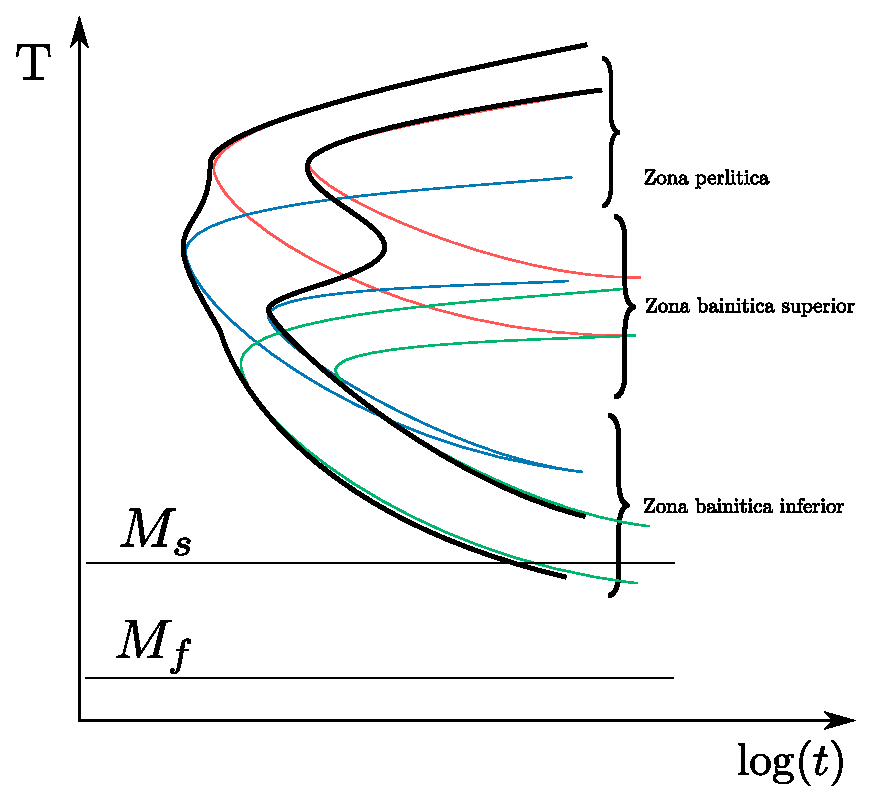
\includegraphics[width=0.7\textwidth]{fig/TTTsuperpuesta.eps}
    \caption{Superposición de curvas perlíticas (rojo) y bainíticas superior (azul) e inferior (verde).}
    \label{fig:TTTsuperpuestas}
\end{figure}

\section[Transformación de la austenita]{Variables que inciden en transformación de la austenita}
Dos variables que inciden en la cinética de estas transformaciones
\begin{itemize}
    \item El tamaño del grano austenítico
    \item La composición química de la austenita que se transforma.
\end{itemize}

Los borde de granos son los sitios de nucleación preferencial para las transformaciones perlítica y bainítica así como para la aparición de las fases proeutectoides ferrita y cementita. Por ende:
\begin{itemize}
    \item Mayor tamaño de grano \goright
    \item[\goright] Menor superficie total de bordes de granos \goright
    \item[\goright] Menor sitios de nucleación \goright
    \item[\goright] Transformaciones comienzan a mayores tiempos
\end{itemize}
\textbf{lo que implica que con mayor tamaño de grano las curvas se mueven a la derecha.}

La composición química juega un rol importante en el efecto sobre $\Delta G$ y $D_c$. Los elementos \textbf{gamágenos} hacen descender la energía libre de la austenita lo que reduce tanto la velocidad de nucleación como la de crecimiento. Los elementos alfágenos hacen subir la fuerza impulsora y en principio deberían acelerar las transformaciones, pero \hl{hacen exactamente lo contrario}.

Porqué sucede esto? En las palabras del profesor (resumidas): Durante la nucleación de ferrita en los borde de grano ocurre que los elementos \textbf{alfágenos} necesitan repartirse hacia la ferrita y los \textbf{gamágenos} necesitan concentrarse en la austenita. Ambos tienen un coeficiente de difusión mucho menor al del carbono y por eso se retrasan las transformaciones de fase.

Además! Los alfágenos son \textbf{formadores de carburos} lo que significa que se tienen que repartir hacia los mismos para que precipiten. Esto también retrasa las transformaciones que involucran precipitación de carburos. 

Algunos elementos simplemente retrasan la difusión del carbono, lo que también retrasa las transformaciones.

Efectos de elementos alfágenos:
\begin{itemize}
    \item Suben \Aone y \Athree (estabilización de ferrita [$\alpha$])
    \item Bajan \Bs, separando las curvas perlíticas y bainíticas
    \item Retrasan más la transformación ferrítica y perlítica que la bainítica. El Molibdeno acelera débilmente la transformación bainítica
    \item El Boro en diminutas cantidades (60ppm) provoca un fuerte retraso en la nucleación de la ferrita proeutectoide. De aquí surgen aceros de alta templabilidad.
\end{itemize}

Efectos de elementos gamágenos:
\begin{itemize}
    \item Bajan temperaturas \Aone, \Athree, \Bs y $M_s$
    \item Retrasan ambas transformaciones (perlita, bainita)
\end{itemize}

\section{Curvas CCT}
\textit{Continuous Cooling Transformation} son curvas representativas de las fases obtenidas a velocidad de enfriamiento constante. Cuando el enfriamiento es continuo desde el campo estable de $\gamma$, el tiempo de comienzo de la transformación no coincide con el que dice la curva TTT. Es porque la austenita pasa por un rango de T donde los periodos de incubación son grandes, de esta forma ``retrasando'' las curvas respecto las TTT.

\begin{figure}[htb!]
    \centering
    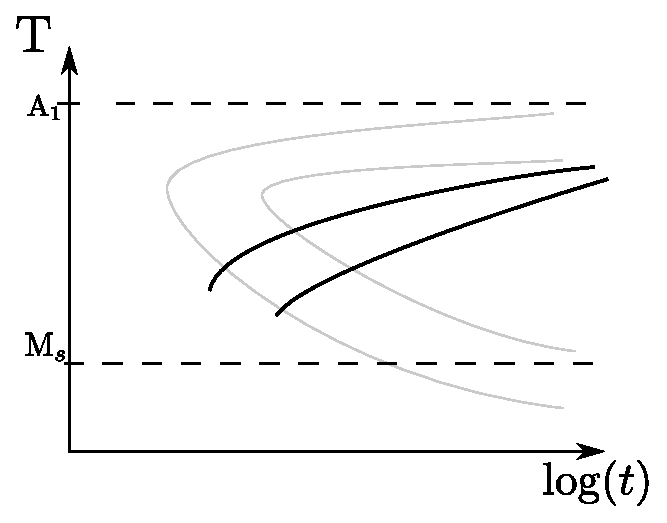
\includegraphics[width=0.8\textwidth]{fig/CCTeutect.eps}
    \caption{Curvas de enfriamiento continuo (CCT) para un acero \textbf{eutectoide}. CCT en negro, curvas TTT en gris claro.}
    \label{fig:CCTeutect}
\end{figure}

\subsection{CCT para un acero hipoeutectoide}
Las curvas de enfriamiento para un acero \textbf{hipoeutectoide} de la figura \ref{fig:CCThipo} pueden ceder las siguientes estructuras y microconstituyentes:\footnote{Tener en cuenta que las curvas rojas de la figura \ref{fig:CCThipo} se dibujan hasta donde haya austenita sin trasformar, es decir, el final de la curva esta donde $\gamma=0\%$.}


\begin{itemize}
    \item[Ciclo 1] Se obtiene ferrita de grano grueso y perlita gruesa en fracciones cercanas al equilibrio
    \item[Ciclo 2] Ferrita de grano mas fino que en el ciclo 1 y perlita fina. Perlita es diluida en ferrita que se encuentra presente en cantidades mayores a la de equilibrio. 
    \item[Ciclo 3] Ferrita, bainita y una fracción de Martensita que sale de la austenita que no se transformo al llegar a $M_s$ \footnote{La curva $M_s$ no es constante para todos los aceros. Si se tiene un acero hipereutectoide, al comenzar a formar bainita la concentración de carbono en la austenita sin transformar va aumentar, reduciendo asi $M_s$ a menor velocidad de transformación por ser un elemento gamágeno.}
    \item[Ciclo 4] Mínima velocidad de transformacion para lograr 100\% de martensita denominada \hl{Velocidad Critica de Temple}
\end{itemize}

\begin{figure}[htb!]
    \centering
    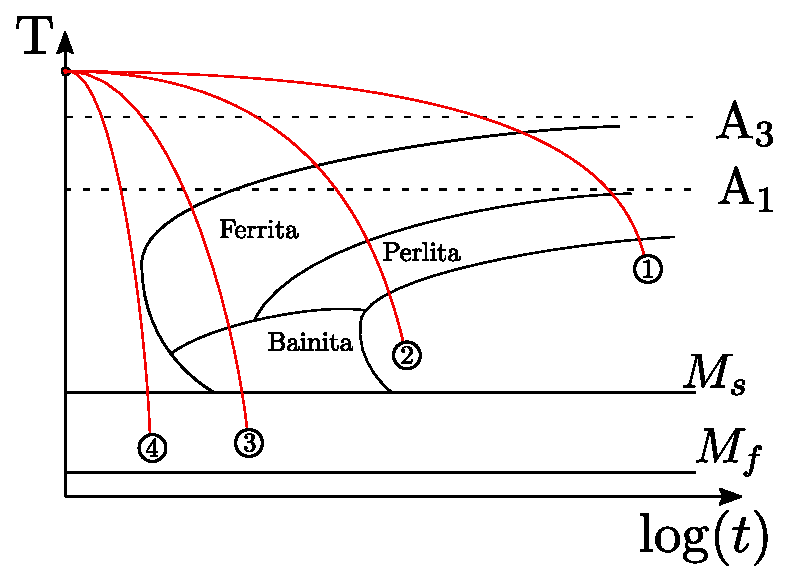
\includegraphics[width=0.7\textwidth]{fig/CCThipo.eps}
    \caption{Curvas de enfriamiento continuo (CCT) para un acero \textbf{hipoeutectoide}.}
    \label{fig:CCThipo}
\end{figure}

NOTA: La curva $M_s$ baja después de un tiempo dado!


\subsection{Variación de propiedades mecánicas con la velocidad de enfriamiento}
Aumentando la velocidad de enfriamiento de la austenita, las transformaciones ocurren en un rango de temperaturas más bajas, logrando microconstituyentes más finos que conlleva con un aumento de dureza y resistencia a la tracción. 

Las estructuras que surgen de un enfriamiento continuo son más complejas que las de transformaciones isotérmicas ya que al pasar por un rango más amplio de temperaturas de transformación se pueden obtener mezclas muy variadas de los microconstituyentes.
% !TeX spellcheck = es_ES
% !TeX root = ../metalurgy.tex
\part{Tratamientos térmicos}
Un tratamiento térmico (TT) es un ciclo térmico aplicado a un metal con el objeto de obtener una cierta combinación de propiedades, también puede usarse para relevar tensiones residuales. La modificación de las propiedades tiene una profunda relación con las transformaciones de fase que ocurren en el metal a causa del ciclo térmico.

Clasificación de TT de aceros:
\begin{itemize}
    \item Sin cambio de composición química
    \begin{itemize}
        \item Volumétrico
        \item Local
    \end{itemize}
    \item Termoquímicos
    \item Hipercrítico $T>$\Athree~
    \item Intercrítico $\Aone<T<\Athree$ o \Acm~
    \item Subcrítico $T<$ \Aone~
\end{itemize}



\section{Austenización}
No es un tratamiento en sí, es la primer etapa de cualquier tratamiento térmico hipercrítico (TTH). Una vez llegado a la temperatura \Athree{} comienza el lento proceso de austenización. Se acelera la transformación con el aumento de la temperatura, pero hay factores que impiden utilizar temperaturas demasiado altas.

\begin{itemize}
    \item \textbf{Costo} aumenta más fuertemente con la temperatura que con el tiempo. (Energía y vida útil de instrumentos)
    \item \textbf{Tamaño de grano austenítico crece} al aumentar temperatura. Trae problemas en propiedades finales y fisuración en TT posteriores
    \item \textbf{Oxidación} aumenta y se propaga al interior del material. Limita uso de materiales de pequeño espesor. Se puede usar una atmósfera protectora.
    \item \textbf{Sobrecalentamiento y quemado} a altas temperaturas (1100\grad). Suele traer problemas para conformado en caliente posterior o para tratamientos de aceros de alta aleación
\end{itemize}

La temperatura a la cual se decide austenizar se llama, apropiadamente, \textbf{temperatura de austenización} ($T_A$) siendo esta mayor a \Athree{} o \Acm{}. $T_A$ surge de un compromiso entre la necesidad de disminuir el tiempo del austenizado y la de evitar los fenómenos antes mencionados. 

$T_A$ varía para cada acero y proceso dependiendo principalmente de
\begin{itemize}
    \item Composición química
    \begin{itemize}
    	\item Para aceros de alta aleaci\'on la cantidad de alf\'agenos aumenta \Athree. $T_A$ puede llegar a los 1300\grad~
    \end{itemize}
    \item Tipo de TT que se aplicara posterior al austenizado
\end{itemize}

El tiempo de austenización depende de
\begin{itemize}
    \item \textbf{Sección máxima} de la pieza ya que el núcleo de la pieza va tardar en tomar temperatura y austenizar. También influye el horno (potencia, capacidad, tipo)
    \item \textbf{Temperatura $T_A$.} Aumenta velocidad de austenización con su aumento
    \item \textbf{Microestructura}: Si se tiene carburos gruesos, zonas segregadas, o una alta aleación estos tardaran en disolverse
\end{itemize}

Cabe destacar que la velocidad de calentamiento no es factor importante para aceros de baja aleación. Estos se pueden cargar en el horno a $T_A$. Para aceros de alta aleación hay varias razones para controlar la velocidad de calentamiento.
\begin{enumerate}
    \item \textbf{Evitar tensiones térmicas.} Aceros de alta aleación tienen mayor coeficiente de dilatación térmica
    \item \textbf{$T_A$ mayor.} Debido a la gran cantidad de alfágenos
    \item \textbf{Mayor \% carbono.} Mayor fragilidad y riesgo de fisuración
    \item \textbf{Geometrías complejas.} Influye en concentración de tensiones térmicas
\end{enumerate}

{\bf Resumiendo}: El objetivo del austenizado es obtener, en el menor tiempo posible, una austenita químicamente homogénea, de tamaño de grano fino y homogéneo, minimizando la modificación de la composición química de la superficie, y reduciendo la distorsión y riesgo de fisuración que pudiera producirse durante el calentamiento o durante la mantención a la temperatura de austenización. 

Es una etapa fundamental para cualquier tratamiento hipercrítico, en especial para aquellos que buscan endurecer el acero. El resultado del tratamiento térmico depende en gran parte de una correcta austenización.

\section{Tratamientos hipercríticos}
Los tratamientos hipercr\'iticos llevan el acero a una temperatura sobre \Athree~ para lograr austenizaci\'on de una gran parte del acero.
\subsection[Recocido de regeneración]{Recocido de regeneración (Full annealing)}
Consiste en llevar el acero a $T_A$\footnote{Para aceros hipoeutectoides suele estar a 20 a 40\grad~ sobre \Athree~} y mantenerlo ahí un tiempo adecuado para asegurar la homogeneidad de la austenita y luego un enfriamiento lento en horno (costoso económicamente) de alrededor de 5 a 50\grad{}/h. Para un acero hipoeutectoide el recocido de regeneraci\'on ser\'ia el camino 1 de la figura \ref{fig:CCThipo}.

\begin{figure}[htb!]
\centering
\begin{subfigure}{0.4\textwidth}
    \includegraphics[width=\linewidth]{fig/TTrecoreg.eps}
    \caption{\textbf{Hipercrítico}.}
    \label{fig:TTrecoreg}
\end{subfigure}
\begin{subfigure}{0.4\textwidth}
    \includegraphics[width=\linewidth]{fig/TTrecoreghiper.eps}
    \caption{\textbf{Intercrítico} para aceros hipereutectoides.}
    \label{fig:TTrecoreghiper}
\end{subfigure}
\caption{TT Recocido de regeneración.}
\end{figure}



Se obtiene una perlita gruesa que conlleva una dureza baja. Si es lo suficientemente lento el enfriamiento se puede obtener perlita parcialmente esferoidizada.

Objetivos:
\begin{itemize}
    \item Reblandecer el acero
    \begin{itemize}
        \item Estructuras de ferrita proeutectoide de tamaño de grano grueso y perlita gruesa, implica mejor formabilidad y maquinabilidad a costo de dureza
    \end{itemize}
    \item Llegar a estructura favorable para el mecanizado y deformación en frió
    \item Obtener otras propiedades finales especificas
    \begin{itemize}
        \item Aplicaciones en industria bulonera para mejorar proceso de recalcado y laminación de roscas
    \end{itemize}
\end{itemize}

El \textbf{recocido de regeneración isotérmico} consiste en realizar la transformación de la austenita a una temperatura constante y relativamente cercana a la de equilibrio. Es mas rápida pero puede dejar el acero con una dureza mayor y requiere de un horno de sales.

\begin{figure}[htb!]
    \centering
    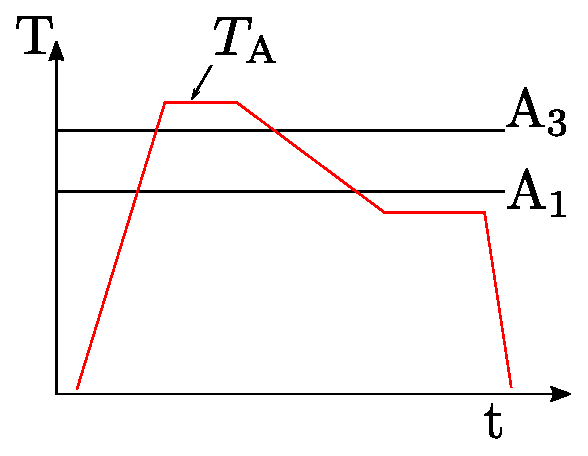
\includegraphics[width=0.5\textwidth]{fig/TTrecoregiso.eps}
    \caption{Recocido de regeneración isotérmico.}
    \label{fig:TTTrecocidoregeneracionisotermico}
\end{figure}

En el caso de los aceros \textbf{hipereutectoides} el tratamiento es \hl{intercrítico} para evitar precipitación de laminas de \cementita~ en los bordes de grano de la austenita.

\textbf{Resumiendo:} el recocido de regeneración es un tratamiento largo y costoso que deja al acero en un estado de baja dureza y alta ductilidad. En aceros de medio y alto C esto es muy conveniente para reducir los costos del conformado plástico en frío y/o del mecanizado. Menos frecuentemente se puede usar para lograr propiedades finales.

\subsection{Normalizado}
Similarmente al recocido, en el \textbf{normalizado} se calienta el acero hasta $T_A$\footnote{Temperatura unos 50 a 80\grad~ sobre \Athree~} y se mantiene para asegurar austenita homogénea y finalmente se \textbf{enfría a aire calmo}\footnote{Velocidad entre 40 a 200\grad{}/min}. Si se busca obtener martensita se denomina \textbf{temple al aire}. El normalizado puede ser tanto un tratamiento intermedio como también un tratamiento final.

\begin{figure}[htb!]
    \centering
    \includegraphics[width=0.5\textwidth]{fig/TTnorm.eps}
    \caption{Normalizado.}
    \label{fig:TTnorm}
\end{figure}

Objetivos:
\begin{itemize}
    \item Homogeneización química y estructural
    \item Refinamiento de tamaño de grano ferritico y de los carburos
    \item Preparar mejor al acero para un tratamiento posterior (dos puntos anteriores)
    \item Mejorar maquinabilidad en aceros bajo carbono
    \item lograr propiedades mecánicas especificas para el servicio
\end{itemize}

La estructura resultante depende de la composición del acero y tamaño de la pieza. En aceros al C y muchos de baja aleación se obtiene ferrita proeutectoide de tamaño más fino que en el recocido y en menor proporción. El resto de la estructura es perlita más fina y en mayor proporción de lo que indica el diagrama de equilibrio. En aceros con transformaciones más lentas pueden aparecer combinaciones de otras fases incluyendo la bainita y martensita.

El normalizado se aplica típicamente a piezas coladas y forjadas en caliente para refinar la estructura de solidificación. Para aceros de bajo \%C se vé un aumento en la maquinabilidad.
\section{Tratamientos subcríticos}

\subsection{Recocido de relevamiento de tensiones}
Consiste en calentar el acero hasta una $T<$\Aone{} y mantenerla un tiempo adecuado para disminuir tensiones residuales y luego enfriar lentamente\footnote{5 a 10\grad/h}.

Objetivos:
\begin{itemize}
    \item Disminuir tensiones residuales
    \item Evitar fenómenos de \textbf{rotura diferida} causados por el hidrógeno o bien algún tipo de corrosión bajo tensión.
    \item Aumentar \textbf{estabilidad dimensional}
\end{itemize}

\subsection{Recocido de globulización}
Consiste en calentar al acero hasta una $T$ por debajo a \Aone~ y mantenerla un tiempo adecuado. Microestructuralmente se busca globulizar los carburos laminares de la perlita.

\begin{figure}[htb!]
    \centering
    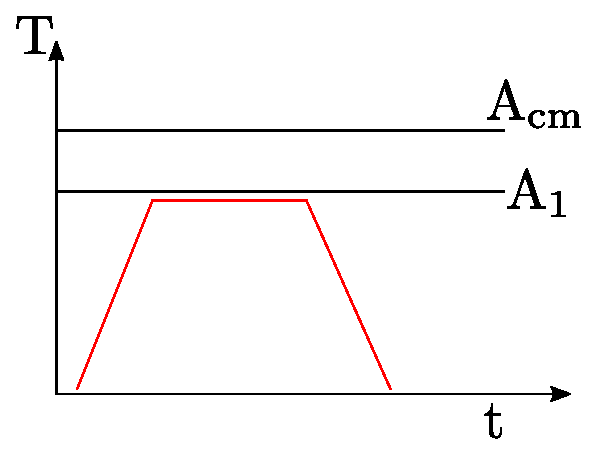
\includegraphics[width=0.5\textwidth]{fig/TTglob.eps}
    \caption{Recocido de globulización \textbf{subcrítico}.}
    \label{fig:TTglob}
\end{figure}

La fuerza impulsora para la esferoidización es la energía de interfaz. Es muy baja y por ende se requiere largos tiempos. Cuanto menor es el espaciado interlaminar de la perlita, mas rápido es el proceso.

Clasificación de estos recocidos, incluyendo las versiones que no son subcríticas:
\begin{itemize}
    \item Subcrítico $T\approx\Aone-50\grad$. Se requiere mucho tiempo. Puede ser acelerado con deformación plástica previa a costo de deformar mi pieza. Es el que se toma en el parcial.
    \item intercrítico $T\approx\Aone+50\grad$. Más corto pero se requiere un estricto control de temperatura y en la velocidad de enfriamiento
    \item Oscilante $T\in\{\Aone-50\grad;\,\Aone+50\grad \}$. Misma ventajas/desventajas que intercrítico.    
\end{itemize}

\section{Temple}

Consiste en austenizar al acero totalmente o parcialmente\footnote{Para acero hipoeutectoides varia entre 40 a 60\grad~ sobre \Athree.} y luego enfriarlo suficientemente rápido para obtener una fracción significativa de martensita (en general no menos de 50\%). 

Clasificación de Temples
\begin{itemize}
    \item Superficial
    \begin{itemize}
        \item Inducción
        \item Llama
    \end{itemize}
    \item Local
    \item Volumétrico
\end{itemize}
Clasificación por método
\begin{itemize}
    \item Por inmersión
    \item Por aspersión o neblina
    \item En matriz metálica refrigerada
\end{itemize}

La \textbf{velocidad critica} es la mínima velocidad de enfriamiento para asegurar 100\% martensita. Es un indicador de templabilidad y esta relacionada con la posición de la nariz de la curva CCT.

El \textbf{efecto de masa} se le dice a la variación de la velocidad de enfriamiento entre distintos puntos de una pieza causada por su inercia térmica. El efecto es mayor a medida que aumenta el tamaño de la pieza.

\subsection[Severidad de temple]{Severidad de temple ($H$)}
Propiedad del medio de temple que indica su capacidad para extraer el calor desde la superficie de la pieza. Una severidad infinita baja instantáneamente la temperatura de la pieza hasta la del baño de temple. La severidad de temple $H$ se mide experimentalmente y depende fuertemente de la composición del medio de temple (que determina sus propiedades térmicas y otras propiedades físicas como la presión de vapor, densidad, viscosidad, etc), de su temperatura y de su grado de agitación. 


\begin{table}[htb!]
\centering
\begin{tabular}{l|l|l|l|l}
\hline
\multicolumn{1}{c|}{\multirow{2}{*}{Agitación}} & \multicolumn{4}{c}{Medio}            \\ \cline{2-5} 
\multicolumn{1}{c|}{}                           & Aire & Aceite    & Agua    & Salmuera \\ \hline
Ninguna                                         & 0,02 & 0,25-0,30 & 0,9-1,0 & 2        \\
Moderada                                        & -    & 0,3-0,4   & 1,0-1,3 & 2-2,2    \\
Acentuada                                       & -    & 0,4-0,5   & 1,4-1,5 & -        \\
Fuerte                                          & 0,05 & 0,5-0,8   & 1,6-2,0 & -        \\
Violenta                                        & -    & 0,8-1,1   & 4       & 5        \\ \hline
\end{tabular}
\caption{Severidad de Temple ($H$)}
\label{tab:severidadTemple}
\end{table}

Lo mejor que hay de medio de temple es salmuera seguido de agua y aceites. Agua a 20 \grad{} tiene un $H=1$ por definición. Los aceites tienen la ventaja de tener velocidad baja en la etapa \ref{item:etapaCEnfriamiento} (secci\'on \ref{ssec:enfriamientoEnMedio}), esto evita fisuras. 

Lo mas deseable es enfriamiento rápido en las primeras etapas y un enfriamiento lento en la etapa \ref{item:etapaCEnfriamiento} para no fisurar la pieza. Se puede cambiar el medio de temple de agua a aceite terminado las primeras etapas pero esto requiere un maestro templador y no se puede hacer de forma industrializada.

La agitación contribuye a la severidad del temple y reduce  duración de la etapa A. También aumenta la velocidad de enfriamiento de la etapa \ref{item:etapaBEnfriamiento} pues ayuda desprender las burbujas de vapor. Genera convección forzada en etapa \ref{item:etapaCEnfriamiento}  aumentando enfriamiento.

Elección de severidad de temple para lograr una cierta dureza $\HB_{\mathrm{deseada}}$
\begin{itemize}
    \item Mayor templabilidad del acero \goright Menor severidad
    \item Si la pieza es grande o el acero no puede llegar a $\HB_{\mathrm{deseada}}$ aun con la mayor severidad de temple posible se deberá usar un acero mas templable
    \item Es necesario evaluar la aplicabilidad de la severidad para disminuir el riesgo de fisuración ya que el calculo de templabilidad no garantiza que se pueda alcanzar $\HB_{\mathrm{deseada}}$ sin fisurar.
\end{itemize}
\textbf{Conclusión:} Necesito alta \textbf{templabilidad} para la mayoría de los casos!

\subsection{Templabilidad}
La \textbf{templabilidad} es la capacidad de una aleación ferrosa (acero o fundición) para obtener martensita a partir de la austenita cuando esta se enfría en condiciones bien definidas. Está relacionada con la cinética de las transformaciones con difusión de la austenita cuando esta es enfriada y por lo tanto con la posición y forma de las curvas de transformación CCT del acero. \hl{Es una propiedad intrínseca y no depende de el tamaño de la pieza o la velocidad de enfriamiento.}
\begin{figure}[htb!]
    \centering
    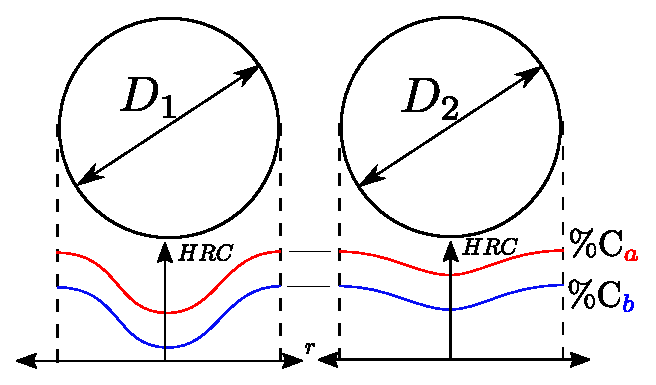
\includegraphics[width=0.6\textwidth]{fig/Templabilidad.eps}
    \caption{Dureza en función de posición $r$ donde $D_1 = D_2$. La probeta 1 es un acero de baja aleación y la probeta 2 es un acero de alta aleación (más templable). Porcentaje carbono ${\color{red} a}> {\color{blue} b}$. }
    \label{fig:templabilidad}
\end{figure}
Los siguientes factores controlan la templabilidad
\begin{enumerate}
    \item Aleantes (con la excepción del cobalto)
    \begin{itemize}
        \item Retrasan las transformaciones con difusión (perlítica y bainítica) aumentando así la templabilidad
        \item Efecto sinérgico entre aleantes significa que conviene mezclar pequeñas cantidades de varios aleantes
    \end{itemize}
    \item Tamaño de grano
    \begin{itemize}
        \item A mayor tamaño de grano se tiene mayor templabilidad
        \item No se usa para aumentar la templabilidad pues conlleva un deterioro en las propiedades finales
    \end{itemize}
    \item Presencia de otras fases
    \begin{itemize}
        \item Presencia de otras fases aumenta sitios de nucleación y acelera transformaciones con difusión
        \item Estas fases pueden retener aleantes
    \end{itemize}
\end{enumerate}


\setcounter{footnote}{0}

\subsection[Diámetro crítico]{Diámetro crítico ($D_0$)}
 Se define como el máximo diámetro en el que puede obtenerse 50\% martensita en el centro cuando se lo enfría con un medio de temple bien definido. Para un $D<D_0$ se tendrá menos de 50\% martensita en el centro.

\textbf{Diámetro critico ideal} $D_{I}$: El diámetro para el cual se obtiene 50\% martensita en el centro de la pieza con \textit{severidad de temple infinita} $H=\infty$, es decir que la superficie de la pieza en contacto con el medio de temple toma la temperatura del medio en tiempo nulo. $D_{I}>D_0$

\subsubsection{Ensayo de Jominy (End-Quench)}
\hl{Se templa una probeta (previamente austenizada) con un chorro de agua en desde un extremo}. Luego se rectifica la probeta \textbf{longitudinalmente} y se mide la dureza en varios puntos, cada uno a una distancia $d_j$\footnote{Se suele denominar distancia de Jominy.} del extremo templado. Las condiciones que afectan la velocidad de enfriamiento también están estandarizadas: velocidad y temperatura del agua, diámetro del caño que conduce el agua hacia el extremo que se templará, y distancia entre este caño y el extremo de la probeta.

\begin{figure}[htb!]
    \centering
    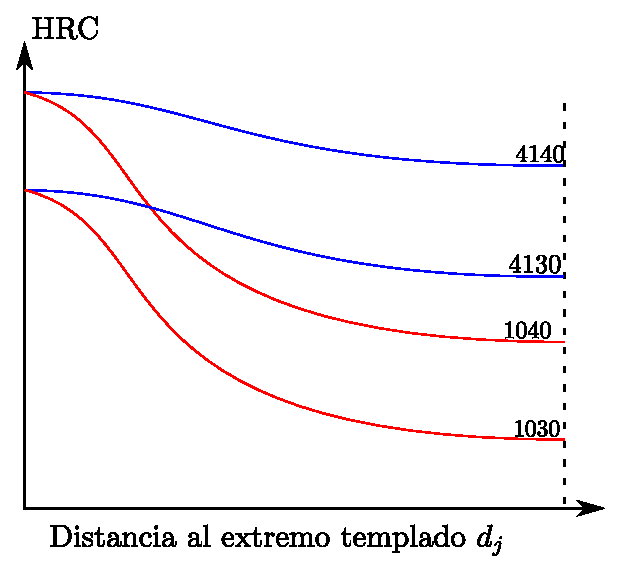
\includegraphics[width=0.7\textwidth]{fig/jominy.eps}
    \caption{Curvas de Jominy para aceros de alta aleación(en {\color{blue} azul}) y para aceros al carbono(en {\color{red} rojo}). A mayor porcentaje de carbono hay mayor dureza en el extremo templado.}
    \label{fig:jominy}
\end{figure}

La ventaja del temple desde un extremo respecto de un temple por inmersión es que se logra un rango de velocidades de enfriamiento muy amplio en una probeta relativamente pequeña. Mientras que el extremo templado se enfría muy enérgicamente ($>200$ \grad/s), el otro extremo sufre algo parecido a un tratamiento de normalizado. Entre estos dos extremos se logran diferentes velocidades de enfriamiento y por lo tanto distintas estructuras y durezas.

\textbf{La curva de Jominy}: Agregar carbono aumenta dureza del extremo templado. Mayor templabilidad achata la curva

\textbf{Templabilidad garantizada:} Cuando la curva Jominy de un acero presenta una dureza dentro de los limites preestablecidos se dice que es un \textbf{acero de templabilidad garantizada} y se le agrega un sufijo a la designación AISI/SAE. Ejemplo: ``SAE 1340 H'' 


Se prefiere una alta templabilidad en los siguientes casos
\begin{itemize}
    \item En piezas de sección grande debido al efecto masa que no permite alcanzar velocidades rápidas en el núcleo de la pieza
    \item Piezas de geometría compleja donde existe alto riesgo de fisuraci\'on. La templabilidad reduce el riesgo de fisuración
\end{itemize}

Los cálculos de templabilidad permiten determinar 

\begin{itemize}
    \item 
\end{itemize}



\subsection{Enfriamiento en medio volátil}\label{ssec:enfriamientoEnMedio}
Se distinguen en tres etapas
\begin{enumerate}[label=(\Alph*)] \label{enum:etapasTemple}
    \item A temperatura de pieza alta se forma una envuelta de vapor sobre la superficie de la pieza. Sin agitación esta envuelta es estable y aísla al metal del liquido. El rango de temperaturas en la que ocurre esta etapa se solapa con aquel en que deben evitarse las transformaciones con difusión para poder obtener martensita, por lo tanto es importante reducir la duración de esta etapa. Se puede reducir esta etapa agregando componentes que reduzcan la presión de vapor (para agua hidróxidos y sales)\label{item:etapaAEnfriamiento}
    \item Una vez reducida la temperatura lo suficiente la envuelta se desestabiliza y se pasa a una etapa donde el calor se extrae principalmente como calor de vaporización. \label{item:etapaBEnfriamiento}
    \item cuando la temperatura baja lo suficiente, se detiene la formación de burbujas de vapor y el calor se extrae por conducción y convección del líquido. La velocidad de enfriamiento vuelve a ser baja. \label{item:etapaCEnfriamiento}
\end{enumerate}



\subsection{Origen de tensiones térmicas durante el temple}
Los conceptos básicos son que la transformación de austenita a martensita es una expansión mientras que el enfriamiento es una contracción. 
\begin{enumerate}
    \item Durante el enfriado ($T_{\mathrm{superficie}}>M_s$) la periferia se \textbf{contrae} mas que el centro ocasionando pequeñas tensiones que se relajan por deformación plástica debido a la alta temperatura. 
    \item Eventualmente la temperatura cae lo suficiente como para que la superficie comience a transformarse ($T_{\mathrm{superficie}}<M_s$) y trata de \textbf{expandirse} pero es restringida por el núcleo generando tensiones de compresión en la periferia y tracción en el núcleo. Aun se pueden relajar las tensiones por deformación plástica.
    \item Si el enfriamiento es lo suficientemente rápido se comenzara a formar martensita en el núcleo ($T_{\mathrm{interior}}<M_s$), traccionando la superficie. Estas tensiones no se pueden relajar por deformación plástica ya que la estructura traccionada es martensita fría, generando así \textbf{distorsiones}, \textbf{tensiones residuales} y en el peor de los casos \textbf{fisuración por temple}.
\end{enumerate}
a todo esto, lo que realmente genera las tensiones térmicas es el gradiente térmico. Si se tiene una pieza pequeña no se va tener mucho riesgo.

Consecuencias
\begin{itemize}
    \item Tensiones Residuales: El revenido puede relajar estas tensiones
    \item Distorsión: Cambio de forma de la pieza. Va requerir un enderezado o mecanizado adicional. Es un problema grave ene piezas esbeltas.
    \item Fisuracion por temple: Es el problema mas grave pues su reparación es poco confiable/económica. Piezas de alto carbono son mas susceptibles (+dureza/fragilidad). Puede ocurrir el fenómeno de la \textbf{fisuración diferida}. Esto consiste en la aparición de fisuras minutos o incluso horas después finalizado el temple. Se puede guardar la pieza ``tibia" (150\grad~ por ejemplo) hasta efectuar el revenido.
\end{itemize}
Los problemas de distorsión y más aún los de fisuración, imponen un límite a la máxima severidad H posible de usar en el temple de una determinada pieza. Cuanto mayor sea el \%C del acero y más compleja o peligrosa la geometría de la pieza, menor será la máxima severidad recomendable para evitar la fisuración. Evidentemente, también será mayor la templabilidad del acero necesaria para alcanzar la dureza requerida en dicha pieza.
Cuando el \%C$>0,4$ no es recomendable aplicar severidades de temple altas ($>0,7$) excepto que se trate de piezas simples y pequeñas.

\textbf{Resumiendo:} La distorsión y el riesgo de fisuración por temple imponen un límite en la severidad de temple máxima aplicable para lograr una determinada dureza, dicha severidad de temple máxima es tanto menor cuanto mayor sea el porcentaje de carbono del acero y más compleja sea la geometría de
la pieza.

\subsection{Martensita revenida}
La estructura resultante de un temple correcto no es apta para casi ningún tipo de servicio debido a su extrema fragilidad, en especial cuando el \%C del acero supera 0,25\%. En consecuencia luego del temple siempre se aplica un tratamiento subcrítico que se denomina revenido.

Uno de los propósitos del revenido es el de aumentar la ductilidad y tenacidad de la estructura de temple. El microconstituyente resultante de este tratamiento se denomina genéricamente martensita revenida y tiene excelentes propiedades de resistencia mecánica y tenacidad cuando las temperaturas de revenido son las adecuadas.

A pesar de su alto costo debido a la necesidad de dos tratamientos térmicos y a la presencia de aleantes en el acero, la estructura de martensita revenida posee varias ventajas fundamentales sobre otros tipos de microestructuras.


Ventajas
\begin{enumerate}
    \item Permite alcanzar niveles de resistencia superiores. Se sacrifica resistencia mecánica (en comparaci\'on con martensita sin revenir) para obtener mayor ductilidad y tenacidad. Aun así la resistencia mecánica obtenida es mucho mayor que la que se puede obtener con estructuras ferrítica-bainítica/perlítica
    \item Relación $\frac{R_{p0,2}}{R_m}$ es mucho mayor para un temple y revenido (0,7-0,95) que para una estructura normalizado (0,55 0,65). En consecuencia la tensión de diseño sera mayor en el caso del temple y revenido
    \item A igualdad de dureza entre una pieza templada\goright{}revenida y una normalizada la temperatura de transición es sensiblemente menor para la pieza templada\goright{}revenida. En el rango de durezas 30 a 45 $\HRC$ la martensita revenida tiene mayor tenacidad.
\end{enumerate}
Nota: No vas a obtener tenacidad buena con un acero 0,5\% carbono. Nunca.

\subsection{Curvas de Lamont (Cálculo de templabilidad)}
Una gráfico de las curvas de Lamont, como la figura \ref{fig:lamont}, relaciona el ensayo de Jominy con el porcentaje de martensita obtenida a una distancia $r$ del centro de una barra de radio $R$. 

\subsubsection{Ejemplo de uso para cálculo de templabilidad}
 Si uno templa una barra de diámetro $D=150$mm a severidad $H=1$ (tabla \ref{tab:severidadTemple}) puede entrar a la figura \ref{fig:lamont} y saber que a una distancia de $r=0,1\cdot R=7,5$mm se tiene una dureza igual a la del ensayo Jominy para ese mismo material a $d_j\approx50$mm. Luego de obtener la dureza \HRC{} de un gráfico similar a la figura \ref{fig:jominy} se puede obtener el porcentaje de martensita en dado punto usando un gráfico de Dureza--\%C--\% Martensita (figura \ref{fig:rockewell}).
 
 

\begin{figure}[htb!]
    \centering
    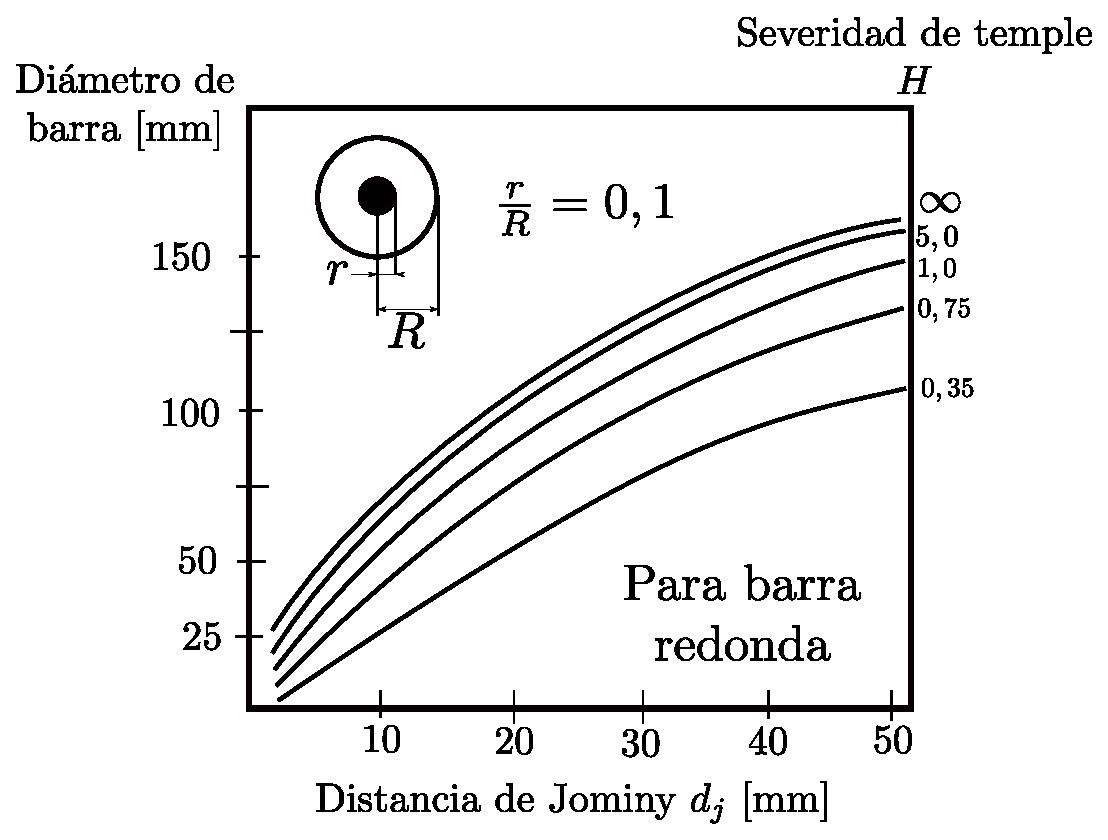
\includegraphics[width=0.8\textwidth]{fig/lamont.eps}
    \caption{Curva de Lamont para una barra redonda $\frac{r}{R}=0,1$.}
    \label{fig:lamont}
\end{figure}


\begin{figure}[htb!]
    \centering
    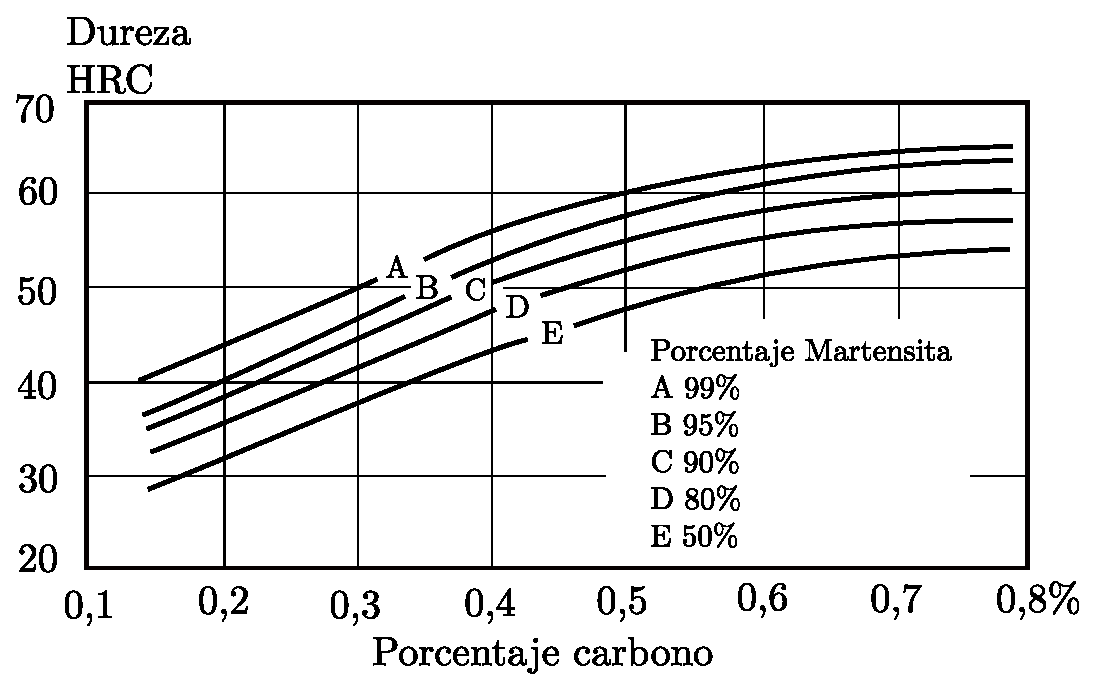
\includegraphics[width=0.8\textwidth]{fig/HRCdiag.eps}
    \caption{Tabla dureza Rockwell tipo `C' (HRC).}
    \label{fig:rockewell}
\end{figure}

\subsection{Temple de aceros hipereutectoides -- Austenita retenida}
\textbf{El temple de aceros hipereutectoides se debe hacer desde temperatura intercrítica.}

La austenita retenida es aquella que, luego del temple, no ha podido transformar a alta temperatura mediante transformaciones con difusión ni tampoco a baja temperatura a martensita. Es lo suficientemente estable a temperatura ambiente como para persistir en la estructura. Sin embargo existen algunas circunstancias que pueden transformarla.

\subsubsection{Variables que influyen en el porcentaje de austenita retenida}
\begin{itemize}
    \item \textbf{Composición química} de la austenita, principalmente \%C. Esto determina rango $M_s$--$M_f$
    \item \textbf{Homogeneidad} del acero (segregaciones)
    \item \textbf{Temperatura} del baño de temple
    \item \textbf{Interrupciones} en el temple. (cambio de medio enfriador)
    \item \textbf{Velocidad de enfriamiento} en el rango $M_s$--$M_f$
\end{itemize}

\subsubsection{Efectos de la austenita retenida}
\begin{itemize}
    \item Disminuye la dureza del temple (en altas proporciones)
    \item Produce \textbf{inestabilidad dimensional} a consecuencia de su posible transformación en servicio, ya sea transformación activada térmicamente a bainita o transformación a martensita activada por tension. En ambos casos la pieza \textbf{aumenta sus dimensiones}. Problema en piezas de tolerancias finas.
    \item Puede producir fallas por \textbf{astillado en filos} cuando transforma a martensita
    \item Cuando se encuentra en bajas proporciones contribuye en el \textbf{fenómeno de fragilización de la martensita revenida} en los aceros al C y de baja aleación.
    \item Si su proporción es baja, su distribución homogénea y fina, y dependiendo de su estabilidad, puede \textbf{aumentar la tenacidad} (aceros al Níquel para uso criogénico, fundiciones ADI, etc).
\end{itemize}

\subsubsection{Métodos para disminuir la cantidad de austenita retenida}
\begin{itemize}
    \item Revenido simple (solo efectivo en el caso de aceros al C y de baja aleación).
    \item Tratamiento criogénico (es caro, tiene altos riesgos de fisuración y requiere tratamientos intermedios de distensionado o revenidos).
    \item Revenidos múltiples (muy usados en el tratamiento de varias clases de aceros para herramientas). Este método puede combinarse con el anterior para mayor efectividad.
\end{itemize}


Proporciones usuales de austenita retenida luego de un temple correcto: 
\begin{itemize}
    \item Aceros al C y de baja aleación, de bajo y medio C: hasta 7\%.
    \item Aceros al C y de baja aleación, de alto C: 5 a 15\%.
    \item Aceros de alto C y alta aleación: 15 a 35\%.
\end{itemize}


\subsubsection{Temple hipercrítico}
Se obtiene principalmente martensita y una fracción alta de austenita retenida, reduciendo la dureza notablemente (puede sobrepasar 50\%). La templabilidad es alta pues todo el carbono y los aleantes están disueltos en la austenita inicial. Sin embargo, por las mismas razones $M_s$ y $M_f$ son bajas y se retiene mucha austenita. Suele ocurrir también con temples intercríticos cercanos a \Acm{}.

Hay riesgo de fisuración por temple por shock térmico.

\subsubsection{Temple intercrítico}
Compuesto principalmente por martensita, \cementita~ globular no disuelta a $T_A$ y una fracción menor de austenita retenida. Tiene templabilidad menor a la de un temple hipercrítico (pues la austenita es menos rica en carbono y aleantes), pero la $M_s$ y $M_f$ son más altas y no se retiene tanta austenita. Si la temperatura de austenización no es muy cercana a \Aone~ la dureza de temple en general es mayor que la del temple hipercrítico (menor \% austenita retenida). 

Si la temperatura es muy cercana a \Aone~ la falta de homogeneidad resultante en la austenita junto con el descenso de templabilidad y el menor porcentaje de carbono de la austenita pueden ser lo suficientemente importantes como para superar los efectos de reducción de la austenita retenida y la presencia de carburos. Debido a esto existe un \textbf{rango de temperaturas intercríticas óptimas} para cada acero hipereutectoide. Por arriba al rango se retendrá mucha austenita y por debajo caerá la templabilidad.

\begin{figure}[htb!]
    \centering
    \includegraphics[width=.9\textwidth]{fig/flowdiagTemple.PNG}
    \caption{Diagrama de flujo para temple. Tener austenita no es para nada grave porque es potencialmente transformable a martensita.}
    \label{fig:flowdiagTemple}
\end{figure}

\section{Revenido}
Es un tratamiento subcrítico que se aplica luego del del temple con el objeto de 
\begin{itemize}
    \item Aumentar ductilidad y tenacidad de la martensita
    \item Lograr propiedades finales del acero
    \item Disminuir tensiones residuales
\end{itemize}

El ciclo térmico consiste en un \textbf{calentamiento} que puede tener varias etapas para evitar el choque térmico para el caso de aceros alta aleación/carbono. Se lleva el acero a la \textbf{temperatura de revenido} $T_R$ la cual varía de acuerdo a las propiedades deseadas ($T_R\in [150, \Aone )$\grad{}).  El \textbf{tiempo de revenido} es el tiempo que la pieza permanece a la temperatura de revenido. El tiempo varía del tamaño de la pieza y de las propiedades finales deseadas, aunque es de menor influencia que $T_R$ (tiempo de 30 min hasta 4 h para piezas tamaño medio). El \textbf{enfriamiento} se efectua en aire calmo excepto en dos casos: 
\begin{itemize}
    \item Cuando se desea disminuir las tensiones residuales se usa una \textbf{baja velocidad} de enfriamiento
    \item Para aceros susceptibles a la fragilización por revenido en cuyo caso se debe enfriar rápidamente en el rango de 580 a 400\grad.
\end{itemize}
\textbf{Revenidos multiples:} En ciertos casos se puede incluir un segundo o tercer calentamiento de $T_R$ igual o levemente diferente. Son usuales para aceros de medio y alto carbono/aleación.

\subsection{Etapas del revenido en aceros al carbono}

\begin{itemize}
    \item[Autorevenido] Ocurre durante el temple. Migración de átomos de carbono hacia zonas de alta densidad de defectos, formando un aglomerado de átomos carbono y/o precipitación de carburos durante el temple. Este fenómeno es más probable y completo a mayor $M_s$ del acero, es decir a bajo carbono\footnote{Ni bien se cruza $M_s$ las primeras martensitas que se forman pasan por un ``mini'' revenido. Este revenido preliminar es más pronunciado a mayor $M_s$.}
    \item[Etapa 1] (100 a 150\grad): Precipitación de carburo $\varepsilon$ ($\mathrm{Fe}_{2,5}\mathrm{C}$ estructura HCP). La precipitación de estas particulas submicroscópicas\footnote{Solo algunos nanometros.} es fina y homogenea causando endurecimiento por precipitación. Esta etapa no aparece en aceros de carbono menor a 0,2\% pues el autorevenido es suficientemente completo para que no haya fuerza impulsora para la precipitación de $\varepsilon$.
    \item[Etapa 2] ($>200\grad$): Transformación de la\textbf{ austenita retenida} a una estructura de ferrita y carburos
    \item [Etapa 3] (a partir de 250\grad): Disolución de los carburos $\varepsilon$ y \textbf{precipitación de cementita} \cementita. Desaparece la sobresaturación de carbono, la martensita deja de existir como una fase BCT y pasa a ser ferrita BCC cuando este problema se completa.
    \item[Etapa 4] (a partir de 300\grad): Coalescencia progresiva de las partículas de cementita. Fuerte descenso de dureza. A mayor temperatura y/o tiempo los carburos tienen mayor tamaño aunque su fracción en volumen permanece constante
\end{itemize}

Si bien no se las considera etapas, hay otros dos fenómenos que pueden
ocurrir a mayor temperatura de revenido.

A partir de los 400\grad~ ocurre la recuperación de las dislocaciones de la
martensita (formación de subgranos dentro de los listones).


A partir de los 600 \grad~ puede ocurrir la recristalización, los listones son
reemplazados por granos equiaxiales.

\hl{La estructura final de un revenido de alta temperatura en un acero al C
está compuesta por granos de ferrita pequeños y más o menos equiaxiales
y carburos finos (del orden de 0,1 micrometros) distribuidos uniformemente. Este
tipo de estructura combina una gran resistencia mecánica con una
muy alta tenacidad. Los carburos finos endurecen, pero su tamaño
pequeño, su forma esferoidal, y su distribución uniforme evitan que se
produzca un descenso muy grande en la tenacidad.}

\subsection[Resistencia al revenido]{Revenido de aceros de baja aleación (Resistencia al revenido)}

Ciertos aleantes participan en la formación de carburos (Cr, Mo, V, etc), sea cementitas aleadas (ortorrómbicas) o bien otros carburos aleados. Este tipo de carburos crece más lentamente que la cementita pues requiere la difusión de los aleantes (más lento que el carbono), así \textbf{ralentizando el revenido}. Por esta razón los aceros aleados se tienen que \textbf{revenir más tiempo o a mayor temperatura}.

También el agregado de aleantes agrega \textbf{complejidad a la secuencia de precipitación} de carburos, lo que puede producir un \textbf{máximo o pico de dureza} a altas temperaturas de revenido.

Los aleantes \textbf{retrasan} la descomposición de la austenita retenida y la recuperación de las dislocaciones de la martensita.



El resultado de todas estas influencia es que la dureza baja más lentamente durante el revenido de un acero con elementos\footnote{Cr, Mo, V, Ti, Nb, etc.} formadores de carburos que en un acero al carbono.

En ese sentido se dice que los aleantes aumentan la \hl{\textbf{resistencia al revenido}}. \cite{guille}

\subsection{Variación de propiedades mecánicas durante el revenido}
En aceros al carbono y de baja aleación al aumentar $T_R$ se produce un descenso en la resistencia mecánica y aumento en la ductilidad y tenacidad. 

El tiempo de revenido tiene menor efecto, aumentar $T_R$ 20\grad~ equivale a triplicar el tiempo de revenido.

Existen curvas ``maestras"{} que se representan en función del \textbf{parámetro de revenido}, teniendosé en cuenta el efecto conjunto de la temperatura y del tiempo de revenido. 

\subsection{Fenómenos de fragilización durante el revenido}
A pesar de la tendencia al aumento de la tenacidad durante el revenido,existen dos fenómenos de fragilización que deben tenerse en cuenta pues deterioran la tenacidad del acero:

\begin{itemize}
    \item \textbf{Fragilización de la martensita revenida}: Consiste en un descenso en la tenacidad durante el revenido en un rango de temperaturas intermedia.
    \item \textbf{Fragilización por revenido}: Consiste en un aumento de la temperatura de transición \Tdf. A pesar de su nombre no es un problema que ocurre en el revenido, pues requiere de tiempos de exposición muy prolongados en el rango de temperaturas de fragilización. Es más bien un problema en el servicio de componentes a alta temperatura.
\end{itemize}

\subsubsection{Fragilización de la martensita revenida}
Fenómeno de fragilización que ocurre durante el revenido de la martensita en el rango de 260 a 400\grad{}. Se produce en los tiempos usuales de un revenido (1h) y afecta tanto aceros al carbono como aleados. Si el revenido se realiza a $T_R>$400\grad el fenómeno no ocurre aunque la pieza sea sometida a temperaturas de fragilización durante su servicio. En este sentido se dice que es \textbf{irreversible}.

Efectos incluye un aumento de \Tdf~ y baja tenacidad. El modo de fractura frágil es intergranular solo en el caso de aceros de baja pureza\footnote{Recordemos que en aceros de baja pureza los carburos nuclean en los bordes de grano formando carburos a base de fósforo, Sb, Sn, As. Esto facilita la propagación de fisuras debido a la baja tenacidad de estos carburos.}, de otro modo es transgranular.

El fenómeno es lo suficientemente rápido como para tener influencia en cualquier revenido que se haga en el rango de susceptibilidad. En el caso en que se requiera alta tenacidad se debe evitar dicho rango. Esto impide obtener una tenacidad alta mediante temple y revenido cuando se requieren durezas altas.

\begin{figure}[htb!]
	\centering
	\includegraphics[width=7cm]{fig/fragilizacionPorRevenidoMartensita.png}\par \vspace{.4cm}
	\includegraphics[width=7cm]{fig/fragilizacionPorRevenidoMartensitaDureza.png}
	\caption{Efecto de la \textbf{fragilización de la martensita revenida}. Gráfico de tenacidad y dureza para un acero 4140 revenido por una hora a varias temperaturas.}
\end{figure}


\textbf{Causas}: el descenso de la tenacidad está asociado a la precipitación de \cementita~ con una distribución y morfología particular durante el revenido. Estas características hacen que se reduzca fuertemente la energía absorbida durante el proceso de fractura. Las impurezas contribuyen por segregación hacia los bordes de grano, pero no son imprescindibles.

\subsection{Fragilización por revenido}
Fenómeno de fragilidad reversible que se produce cuando ciertos aceros se exponen prolongadamente o se enfrían lentamente en el rango de 400 a 580\grad{}. No debe confundirse con la fragilización de la martensita revenida (que se da a menor temperatura) o con la fragilización por creep (que se da a mayor temperatura).

Son susceptibles los aceros aleados de pureza comercial ($>0,6\%$ Mn) y los que tienen elevado contenido de impurezas: Sb, Sn, As, P. Ciertos aleantes aumentan la susceptibilidad, sobre todo si se encuentran combinados: Si, Mn, Cr-Ni, Cr-Mn. El molibdeno (Mo) y el tungsteno (W) bajan las susceptibilidad cuando se encuentran en pequeñas cantidades.

También es importante considerar este efecto para cuando se efectúan revenidos a grandes piezas a temperaturas mayores pero que se enfrían lentamente en el rango de fragilización. Se tiene que considerar que tal vez cierto componente esté trabajando dentro del rango de fragilización (rotores de turbinas de vapor de baja presión, algunos recipientes a presión).

Los \textbf{efectos incluye}
\begin{itemize}
    \item Aumento \Tdf~
    \item El modo de fractura frágil es intergranular
    \item Ciertos reactivos atacan los antiguos bordes de grano austeníticos
\end{itemize}

\textit{Teoría de la doble segregación} como \textbf{causa:} Las impurezas mencionadas segregan en los borde de grano austeníticos en el rango de temperaturas (400 a 580\grad) causando un descenso de la cohesión de los mismos. Este descenso eleva \Tdf~ y favorece la fisuración intergranular frente al modo de fractura frágil transgranular por clivaje. 

Esta teoría explica porque solo los aceros con ciertos aleantes son susceptibles y también porque la fisura avanza por los antiguos bordes de grano austeníticos y no por los borde de grano ferríticos.


\subsubsection{Medidas contra la fragilización por revenido}

\begin{itemize}
    \item Agregado de un bajo \% Mo retrasa fuertemente cinética de la fragilización
    \item Adecuada elección de los aleantes
    \item Reducción de impurezas
    \item Reducción de tamaño de grano austenítico, lo que no es tan fácil en piezas grandes
    \item En los casos de piezas que no trabajan en el rango de fragilización se \textbf{enfría rápidamente desde $T_R$}
    \item Se pueden recuperar piezas fragilizadas en servicio con un tratamiento de revenido $T_R>600$\grad.
    \item Monitoreo de la \Tdf~ en equipos que operen en el rango de fragilización. Técnicas no destructivas de monitoreo.
\end{itemize}

\subsection{Revenidos de alta y de baja temperatura}

La existencia del fenómeno de fragilización de la martensita revenida,
junto con la tendencia al aumento de la tenacidad que ocurre tanto a
temperaturas inferiores a las del rango de fragilización como a
temperaturas superiores al mismo, hace que existan dos rangos de
revenido bien definidos.
Los revenidos de \textbf{baja temperatura} (usualmente hasta unos 250 ºC) se
usan cuando es imprescindible retener una dureza muy alta en el acero,
lo cual implica un sacrificio de la tenacidad. El revenido en este rango
de temperaturas releva parcialmente las tensiones residuales del temple.
Los revenidos de \textbf{alta temperatura} (T>500 ºC) hacen que baje
sensiblemente la dureza de temple en el caso de los aceros al C y de baja
aleación, pero logran una excelente tenacidad con muy buena resistencia
mecánica.


\subsection{Revenido de microconsituyentes no martensiticos}

Al ser estructuras más estables, la velocidad de revenido de la perlita y
las bainitas es bastante inferior a la de la martensita.
En el revenido de la martensita, la mayor pérdida de dureza se da a causa
de la extracción del C en solución sólida sobresaturada y su precipitación
como carburo. En la perlita y la bainita esto no sucede.
En la bainita sólo ocurre un engrosamiento progresivo de los carburos y
una recuperación de las dislocaciones de la ferrita. Ambas cosas
conducen a una disminución de la dureza pero a un ritmo menor que en el
revenido de la martensita.
En el caso de la perlita el proceso de revenido es aún más lento, pues sólo
involucra la esferoidización progresiva de los carburos laminares. Tal
como ya se ha visto este proceso es muy lento.

La diferencia de velocidad con la que decae la dureza durante el revenido de las diferentes estructuras tiene la
importante consecuencia de
que el gradiente de durezas
que se produce luego del
temple, disminuye durante
el revenido, en especial para
altas temperaturas de
revenido.

\section{Martemperado}

Es un temple en dos etapas.
\begin{enumerate}
	\item El acero es enfriado hasta una temperatura ligeramente superior a $M_s$ y allí se mantiene hasta que homogenice su temperatura. Se mantiene 100\% contenido de austenita
	\item En la última etapa el acero es enfriado a una velocidad más lenta pasando por el rango $M_s$ y $M_f$.
	\item[Bis.] Se suele requerir un revenido posterior
\end{enumerate}
la temperatura a la cual se homogeneiza la pieza se denomina la temperatura de martemperado. El tiempo de mantención puede variar mucho (pocos segundos hasta 40 minutos)

No es la solución para adquirir más dureza o templabilidad, solo disminuye el riesgo de fisuración. Igual se requiere un revenido posterior. Se requiere una templabilidad mínima para poder aplicar martemperado y te limitan los espesores de las piezas a tratar.

\subsection{Ventajas}
\begin{itemize}
	\item Disminución de varios efectos incluyendo distorsión, tensiones residuales (macroscópicas) y riesgos de fisuración por temple. Es especialmente recomendado para aceros alto C y piezas esbeltas/complejas
	\item Mejoramiento de propiedades mecánicas respecto temple común (mayor ductilidad y tenacidad a igual resistencia mecánica)
	\item Permite realizar operaciones de enderezado luego de extraer la pieza del baño de martemperado y antes de que se transforme a martensita (aún sigue siendo austenita, asegura alta ductilidad y baja resistencia mecánica)
\end{itemize}



\subsection{Limitaciones}
\begin{itemize}
	\item El enfriamiento inicial es lento y requiere cierta templabilidad mínima. Como regla general solo aceros templables en aceite pueden ser martemperados
	\item Existe una limitación en espesores de las piezas a tratar (templabilidad mínima). Solo se pueden martemperar piezas de espesor grande si son de acero de alta templabilidad. Se puede agregar agua la medio o utilizar una temperatura de martemperado inferior a $M_s$ para aumentar el espesor permisible
\end{itemize}

\subsection{Aplicaciones del martemperado}
Se puede aplicar el martemperado a una gran variedad de piezas con geometría relativamente compleja y espesores no muy grandes hechas de aceros de baja aleación.

Se reduce el riesgo de fisuración en aceros de alto contenido de C y es de interés para piezas carburadas, y aceros de alta aleación donde es posible martemperar grandes secciones de piezas complejas. 



\section[Austemperado]{Austemperado (Austempering)}

Tratamiento isotérmico en el rango de la transformación bainítica. Se enfría el acero lo suficientemente rápido para evitar transformaciones de fases a temperaturas altas hasta llegar a una temperatura mayor a $M_s$ y se lo deja ahí hasta completar la transformación bainítica inferior.

No se austemperan aceros con transformación bainítica lenta ($>60$ minutos) ni los que no cumplan con la templabilidad mínima. La transformación ocurre alrededor de los 260\grad~ a 400\grad~ dependiendo del tipo de acero y nivel de resistencia deseado con un tiempo de mantención entre 5 a 60 minutos. Se suelen usar sales fundidas.

\subsection{Ventajas}
\begin{itemize}
    \item Se disminuye la distorsión, tensiones residuales y probabilidad de fisuración respecto temple y martemperado
    \item Tratamiento corto y económico para producir durezas en el rango 35 a 55 HRC pues no se requiere revenido posterior
    \item A diferencia del martemperado, el tiempo de permanencia en el baño de sales no afecta drásticamente las propiedades finales
    \item En el rango de durezas 45 a 55 HRC la bainita inferior posee aún mejor tenacidad que la martensita revenida a igualdad de durezas (esta tendencia se revierte en el rango HRC 35 a 45)
\end{itemize}

\subsection{Limitaciones}
No se puede aplicar a cualquier aceros por requerimientos de templabilidad. Las limitaciones son mayores que en el martemperado dado que el medio en el cual se enfría tiene una temperatura mayor a la del martemperado lo cual implica una velocidad de enfriamiento más lento.

El tiempo necesario varía dependiendo del acero. En ciertos casos el austemperado tarda mucho tiempo y no es viable economicamente. Además no se pueden alcanzar durezas superiores a 55 HRC, aún en aceros alto C.
% !TeX spellcheck = es_ES
% !TeX root = ../metalurgy.tex
\part{Aceros para construcción Mecánica}
Para fabricación de piezas de maquinaria. Cadena cinemática, transmisión de potencia, elementos roscados, herramientas manuales, industria automotriz, agrícola, aeronáutica, ferroviaria, etc.

Los \textbf{requerimientos de servicio} para un acero incluye propiedades mecánicas como $R_m$, $R_{p0,2}$, tenacidad, resistencia a la fatiga, resistencia al desgaste, resistencia a cargas de contacto. Luego se pueden exigir \textbf{caracteristicas de fabricación} como formabilidad, maquinabilidad y ductilidad. Los requerimientos de servicio y características de fabricación suelen obtenerse de tratamientos térmicos.

\section{Clasificación}

Existen varios tipos de clasificaciones de aceros para contrucción mecánica:

\subsection*{Según aleantes}
\begin{description}
	\item[Aceros al C] Más baratos, fácil fabricación y de menor templabilidad
	\item[Ac. de baja aleación] Buena templabilidad, menor severidad de temple requerida, buena maquinabilidad, buena resistencia al revenido
\end{description}


\subsection*{Clasificación por \%C}
\begin{description}
	\item[Bajo C ($<0,25\%$)] Para cementación/carburización (engranajes, árboles, cadenas)
	\item[Medio C ($0,25 \textrm{ a }0,5\%$)] Aceros para bonificado. Durezas $\approx 30$ a $40$ HRC
	\item[Bajo C ($>0,5\%$)] Máxima resistencia y dureza. Se usan bonificados, martemperados+revenidos, austemperados. Costo alto de fabricación de piezas por baja maquinabilidad y formabilidad.
\end{description}

\subsection*{Clasificación por templabilidad}
Puede ser baja, media o alta. El requerimiento de templabilidad va estar en función a la solicitación.

\begin{description}
	\item[Tracción/corte puro] 90\% mínimo de martensita en el centro. $R_{p0,2}>1200$ MPa. Bulones y tornillos de alto grado
	\item[Flexión/Torsión pura] 50\% martensita en el centro. Árboles, ejes y resortes
\end{description}

\section{Resistencia a la fatiga}
Se determina con un ensayo en la maquina de Moore (flexión rotativa $\sigma_m=0$;$\sigma_a = |\sigma_{\max}|$) definiéndose así las zonas de bajo y alto ciclado.

\subsection*{Como maximizar la resistencia a la fatiga}
En aceros al C de baja aleación con dureza 45 HRC se cumple que $R_f \approx 0,35 - 0,6R_u$ (Shigley toma $0,5R_u$). Esto es valido para una probeta lisa sin tensiones residuales bajo flexión alternativa.

Si se tiene una entalla
\[
q = \frac{k_f -1}{k_t - 1}
\]
$q$ indica cuanta tensión es relevada. $q=1 \Rightarrow$ muy sensible a la entalla.  Para maximizar la resistencia a la fatiga se necesita alta ductilidad y alta $R_m$. Se puede obtener por temple y revenido, o austemperado.

\section{Aceros al boro}
El boro promueve templabilidad a bajo costo en aceros de bajo y medio carbono. El boro (intersticial en la austenita) segrega a los bordes de grano retrasando la nucleación de ferrita proeutectoide. Se corren las curvas CCT a la derecha, ganándose mejor templabilidad.

El boro se puede encontrar en estos aceros en solución sólida, como óxido, nitruros, boruros. Se corre el peligro que al agregar demasiado boro vaya a formar un compuesto que no cumpla ser soluto.

\section{Aceros de corte libre}

Son aquellos con algunos elementos (P y S en general) que se usan cuando la pieza requiere mucho mecanizado y el costo es más importante que las propiedades finales. El azufre hace que se entrecorte la viruta y funcione como lubricante.  El fósforo en solución sólida hace que se fragilice la ferrita logrando viruta entrecortada. SAE 1100$\rightarrow$S; SAE 1200$\rightarrow$S,P.

% !TeX spellcheck = es_ES
% !TeX root = ../metalurgy.tex
\part{Aceros inoxidables}

% \includegraphics{schaeffler.png}

\begin{figure}[htb]
	\centering
	\includegraphics[width=0.6\linewidth]{fig/schaeffler.png}
	\caption{Diagrama de Schaeffler.}
	\label{fig:schaeffler}
\end{figure}



Grupo de aceros de alta aleación diseñados para tener resistencia a la corrosión en un amplio rango de servicio y alta resistencia en un rango amplio de temperaturas.

Las aplicaciones principales de estos aceros son en plantas generadoras de energía, centrales hidráulicas, plantas petroquímicas, industria farmacéutica, piezas de maquinas, arquitectura (decoración), aplicaciones marítimas.

Se pueden clasificar en dos tipos principales
\begin{description}
	\item[Austeníticos] Son los aceros inoxidables de mayor uso debido a la combinación de sus propiedades mecánicas y su alta resistencia a la corrosión
	\item[Ferríticos] Se usan mucho menos que los austeníticos pero poseen algunas ventajas como menor costo y mayor resistencia a la corrosión bajo tensión
	\item[Martensíticos] Son los de mayor resistencia mecánica pero menor resistencia a la corrosión
	\item[Duplex o austenoferríticos] Son el tercer grupo más utilizado , poseen buena combinación de propiedades mecánicas y resistencia a la corrosión
	\item[Endurecibles por precipitación] Comprenden a los Austeníticos, semiausteníticos y martensíticos  
\end{description}

\section{Corrosión}
Deterioro de un material por la acción química del medio que lo rodea. A excepción de los nobles, los metales son termodinámicamente inestables al contacto con el aire y forman óxidos. Si la reacción es ``lenta"{} (desde un punto de vista cinético) la corrosión puede llegar a aceptarse. Si es ``rápida"{} y limita la vida del componenta surgen problemas de costo y fiabilidad mecánica.

\subsection{Clasificación}
\begin{description}
	\item[Generalizada] A nivel macroscópico, la superficie es atacada uniformemente. Es predecible y controlable. Se puede prevenir si se diseña con un sobre-espesor uniforme. El daño es proporcional a la cantidad de material removido.
	\item[Localizada] Daño localizado progresa rápido. Resulta difícil predecir, controlar y detectar. El daño puede ser muy grande aunque la cantidad de material sea mínima. Es muy problemático. A continuación se tienen 4 tipos de corrosión localizada:
	      \begin{description}
		      \item[Picado/Pitting] Promovido por la presencia de iones $Cl^{-1}$, alta temperatura y baja velocidad de circulación del fluido. Si la capa pasivante se rompe localmente y no se forma rápido otra la corrosión avanza y se genera pozos en forma de túneles que pueden perforar el material en corto tiempo aumentando el riesgo de avance de fisura por fatiga. El Cromo, Molibdeno y nitrógeno aumentan la resistencia al picado según el \textbf{índice de picado}: $IP=\% \textrm{Cr} + 3,3\% \textrm{Mo} + X \%\textrm{N}$,  donde $X$ es 0\footnote{El nitrógeno es prácticamente insoluble en la ferrita a temperatura ambiente.}, 16 o 30 para inoxidables ferríticos, duplex o austeníticos, respectivamente. 
		      \item[Rendijas] Se da en zonas donde el fluido no llega a circular debido a la geometría/orientación de la pieza. Cuando se consume el oxigeno se forma una \textbf{celda de aereación diferencial} entre la rendija y el resto de la superficie metálica. Evitable con buen diseño de pieza, reduciendo iones de cloro y reduciendo la temperatura. El Molibdeno mejora la resistencia ante este tipo de corrosión.
		      \item[Bajo tensión] Puede dar lugar  fallas catastróficas a partir de fisuración provocada por la combinación del \textbf{medio} y \textbf{tensión de tracción}. Em general la fisura rompe por fractura frágil. Los aceros inoxidables austeníticos y martensiticos son los más susceptibles. Los aceros austeníticos y martensíticos son los más susceptibles. Hay dos tipos de SCC (Stress  corrosión cracking) más conocidos
		      \begin{description}
				  \item[SCC Fisuración transgranular ramificada] Producido por soluciones con \textbf{cloruros} a temperatura mayor a 60\grad. Agravado por mayor cantidad de cloruros, deformación plástica previa, mayor temperatura y un pH entre 3 y 8.
				  \item[SCC Fisuración intergranular] Causado por soluciones cáusticas de no menos de 20\% concentración a alta temperatura (>130\grad)
			  \end{description}
		      \item[Granular] Asociada a fenómeno de precipitación de carburos ricos en Cr en los bordes de grano de las microestructuras.
	      \end{description}
\end{description}


\subsection{Pasividad}
La pasivación de un metal se refiere a la formación de una delgada capa de óxido al ser sometido a un diferencial de potencial ($\Delta V$) mayor al potencial de pasivación. Esta capa aísla al metal del medio y hace que disminuya la velocidad de corrosión en varios ordenes de magnitud. Para que sea efectiva la capa esta debe ser fina, continua, no porosa, insoluble en el medio, y debe poder regenerarse rápidamente al ser dañada (ralladura, mecanizado). 

El aluminio, por ejemplo, no es electronegativo pero es fuertemente pasivado. El hierro puede pasivarse pero a un alto $\Delta V$. La inclusión de cromo (Cr) en un 12\% o más hace que el metal pueda oxidarse fácil

\subsubsection*{Variables en la estabilidad de la capa pasivante}
\begin{description}
	\item[Composición química del acero] Factor principal es el contenido de Cr (12\% mínimo) para pasivar con soluciones acuosas neutras. En general la heterogeneidades (segregaciones, precip. de carburos) hacen que disminuya la estabilidad.
	\item[Composición del medio] Los inoxidables se pasivan solo cuando el medio es altamente oxidante (acuosos, $HNO_3$). La presencia de iones de halógenos (CL$^{-1}$) desestabilizan la capa pasivante generando corrosión localizada y son es la principal razón por fallas. Un medio básico (pH alto) es más estabilizante para una capa pasivante.
	\item[Variables operativas] En general, la resistencia a la corrosión disminuye con el aumento de la temperatura. La velocidad relativa entre el medio y la superficie afecta la formación de la capa. A mayor velocidad hay mayor aporte de $O_2$, aumentando la velocidad de oxidación y estabilidad de la capa (mientras que no haya fenomeno de erosión--corrosión). Una velocidad alta de circulación puede también prevenir que decanten partículas que catalizen la corrosión.
	\item[Factores de diseño] La presencia de rendijas o alta rugosidad crean zonas que favorecen la oxidación localizada.
\end{description}

\section{Aceros inoxidables austeníticos}
Se trata del grupo de aceros inoxidables que mejor combina propiedades mecánicas y tecnologías con resistencia a la corrosión a precio razonable. Constituyen 70\% de la producción total de aceros inoxidables. 



El Cromo es un elemento alfágeno y consecuentemente no podrían existir aceros inoxidables austeníticos con Cr solamente. Es necesario recurrir a un elemento \textbf{gamágeno}. La composición típica de un acero austenítico inoxidable :
\begin{description}
	\item[Cr] 16 a 30\%
	\item[Ni] 8 a 30\%
	\item[Mo] Hasta 4\%
	\item[Mn] $\approx$ 2\%
	\item[C] Menor de 0,1\%
\end{description}

\subsection{Ventajas de una estructura FCC}
El costo de obtener un acero inoxidable austenítico puede ser justificado según
\begin{itemize}
	\item La gran ductilidad y baja tensión de fluencia por poseer 12 sistemas de deslizamiento. Se traduce en una alta capacidad para el conformado plástico, especialmente en frío.
	\item Los metales monofásicos FCC no poseen \Tdf~ (transición dúctil-frágil) y además poseen alta tenacidad, la cual conservan a hasta bajas temperaturas ideal para aplicaciones criogénicas.
	\item Estructura FCC es inherentemente más resistente a la fluencia a alta temperatura (creep) debido a la menor energía de falla de apilamiento comparado a estructura BCC.
	\item Intersticiales tienen mayor solubilidad y menor difusividad. Esto ralentiza la precipitación de carburos ricos en Cr y en ciertas condiciones lo evita. Estos carburos deterioran la resistencia a la corrosión como veremos
	\item En sistema Fe-Ni-Cr la estructura FCC es amagnética.
\end{itemize}



\subsection{Elección de gamágeno}
El Cr es un elemento alfágeno, entonces se necesita de un gamágeno para estabilizar la austenita a temperatura ambiente.
\begin{description}
	\item[C] Debe ser bajo porque favorece la precipitación de carburos de Cr, lo cual favorece la corrosión
	\item[N] No se usa ya que no estabiliza la austenita hasta bajas temperaturas
	\item[Mn] Se usa en casi todos los austeníticos pero no es el gamágeno principal. Estabiliza la austenita a temperatura ambiente pero no baja tanto $M_s$. La austenita rica en Mn no posee tan buenas propiedades mecánicas como el sistema Fe-Ni.
	\item[Ni] Estabiliza austenita hasta bajas temperaturas. Baja la $M_s$ (reduciendo la formación de martensita, cosa indeseable), mejora la tenacidad y aumenta la resistencia a la corrosión. A mayor cantidad de Cr, Mo y otros alfágenos se requiere de mayor Ni para balancear la estructura y lograr que sea austenítica. La desventaja principal es su \textbf{costo} elevado.
\end{description}

El acero inoxidable en el cual todos los demás están basados tiene la composición 18\% Cr -- 8\% N -- 0,15\% C y algo de Mn. A temperatura ambiente este acero tendría una estructura parcialmente austenítica con algo de ferrita y además carburos de Cromo. La austenita no transforma a martensita pues la $M_s$ es muy baja a consecuencia del contenido de aleantes, en particular el Ni.

A temperatura ambiente un acero inoxidable austenítico contiene muy poca martensita por el $M_s$ bajo, poca ferrita y algunos carburos.

\subsection{Precipitación de carburos de Cromo}
\label{ssec:sensibilizacion}
El \%C aumenta la temperatura a la cual precipitan los carburos del Cromo y la acelera. Los carburos de Cromo nuclean en los borde de grano y bordes de maclas de la austenita. Alrededor de los carburos queda una zona empobrecida en Cr, lo cual lleva a la \textbf{sensibilización}. El impacto se debe al alto contenido de Cromo por carburo M$_{23}$C$_6$ (+70\% en peso).

La sensibilización da origen a la \textbf{corrosión intergranular} y ocurre frecuentemente en aceros austeníticos ya que cuando hay un proceso de alta temperatura el carbono se disuelve y re-precipita al enfriarse.
ralentiza. 

\subsubsection{Causas}
Cualquier proceso que someta al acero a altas temperaturas y posteriormente \textbf{no lo enfrie suficientemente rápido} como para evitar la precipitación de carburos de Cromo, conducirá a un estado sensibilizado. El grado de sensibilización dependerá del contenido de C del acero y la velocidad de enfriamiento.

\begin{itemize}
	\item Soldadura
	\item Tratamientos térmicos
	\item Solidificación
	\item Conformado en caliente
\end{itemize}

\subsubsection{Métodos para revertir la sensibilización}

\begin{description}
	\item[Temple de solución o Hipertemple] Temperatura entre 1010 y 1120\grad y luego un medio de enfriamiento que aporte la velocidad necesaria para prevenir precipitación de carburos de Cr. Limitado por espesor de pieza y distorsión permisible
\end{description}


\subsubsection{Métodos para prevenir la sensibilización}

\begin{description}
	\item[Disminución de \%C]  Grados de aceros 304L, 316L de bajo C ($\leq0,03\%$C) tienen un efecto notable comparado a sus contrapartes 304 y 316 ($\approx 0,08\%$C). La disminución del C retrasa la precipitación y disminuyen su cantidad. Bajo ciertas condiciones estos grados pueden ser soldados sin necesidad de un tratamiento de temple de solubilización posterior. Por otro lado la disminución del C permite aplicar el temple de solución facilmente si fuera necesario. Muy usado en piezas de alto grosor. 
	\item[Agregado de elementos estabilizadores] Nb, Ti, Ta. Grados \textbf{AISI 321, 347 y 348}. Estos elementos forman carburos facilmente y compiten con el Cr, así disminuyendo o evitando la precipitación de carburos de Cr. Para algunos grados se aplica un \textbf{tratamiento de estabilización} en el cual se calienta el acero en un rango de temperatura donde precipitan los carburos de los elementos estabilizadores y en cam,bio es lenta la precipitación de los carburos de Cr (850-900\grad varias horas)
	\item[Composición química] La composición química de estos aceros posee una cantidad de Cr no menor al 16\%. A medida que se agrega Cr, o bien se agrega Mo, se mejora la resistencia a la corrosión y sensibilización. Sin embargo esto debe compensarse con una cantidad adecuada de Ni para poder obtener una estructura austenítica minimizando la presencia de ferrita $\delta$. El \textbf{C} se debe mantener bajo (usualmente <0,08\%) para disminuir la sensibilización. Los grados de bajo C poseen un máximo de 0,03\%. El \textbf{Ti, Nb y Ta} se usan en pequeñas proporciones como estabilizadores en algunos grados. El \textbf{Al, Si y Cu} se agregan en ciertos grados especiales para aumentar la resistencia a algún tipo de corrosión u oxidación en caliente. El \textbf{Mn} está presente en todos los grados (aproximadamente en un 2\%)   
\end{description}

\subsection{Propiedades mecánicas}

\subsubsection{Endurecimiento}
A pesar de su baja tensión de fluencia, se puede decir que los aceros austeníticos presentan las mejor combinación de propiedades mecánicas. En estado de temple de solución, los aceros austeníticos tienen una $\sigma_y$ entre \textbf{200 y 300MPa}, la cual es comparable a un acero común laminado en caliente de 0,1\% o 0,2\% C (AISI 1010, 1020). La tensión de fluencia es una gran desventaja pues los métodos de endurecimiento son restringidos pues no deben afectar demasiado a la resistencia a la corrosión.

El \textbf{refinamiento de grano} no es tan fácil de lograr como en aceros al carbono. No puede lograrse por tratamiento normalizado, pues no existe cambio alotrópico $\alpha \rightarrow \gamma$. Aplicando deformación en frío y luego un recocido se reduce el tamaño del grano apreciablemente. Surge un problema en este último tratamiento: el rango de temperaturas del recocido cae dentro del rango de precipitación de carburos de Cr. Por otra parte el \textbf{coeficiente $k_y$ de la ecuación Hall-Petch es aproximadamente la mitad que para aceros ferríticos} de modo que es menos efectiva la reducción en tamaño de grano que en aceros ferríticos de baja aleación.

El \textbf{endurecimiento por precipitación} se usa en algunos aceros inoxidables austeníticos, como así en semiausteníticos y martensíticos. Estos aceros austeníticos tienen mayor resistencia mecánica ($R_{p0,2}$ entre \textbf{500 y 900MPa}). En general el precipitado no involucra al Cr ni C, si no otro tipo \textbf{intermetálico}. De modos estos aceros tienen más problemas de fabricación (conformado/soldadura) que los austeníticos comunes y son más costosos de tratar térmicamente. Por todo esto su uso es más restringido que el austenítico inoxidable. 

Los aceros inoxidables austeníticos son principalmente \textbf{endurecidos por deformación en frío} debido a estos últimos puntos. El coeficiente de endurecimiento por deformación de estos aceros es muy alto pues poseen baja EFA.

En los aceros inoxidables austeníticos, durante la deformación plástica en frío se puede transformar algo de austentíta en martensita si es que la $M_d$ es suficientemente alta. La martensita eleva la resistencia y aumenta el coeficiente de endurecimiento por deformación. El elemento que más influye en esto es el Ni. Aceros con alto contenido de Ni poseen baja $M_d$ y se denominan \textbf{estables} ya que no transforma casi nada de austenita en martensita durante la deformación a temperatura ambiente. Otros aceros austeníticos inoxidables con menor cantidad de Ni presentan mayor transformación de martensita y se denominan \textbf{inestables.}

Dependiendo del proceso de conformado en frío, se puede desear un bajo coeficiente de endurecimiento por deformación (procesos de altas tensiones de compresión, ej. recalcado, laminación de roscas) o uno alto (procesos con tensiones uniaxiales o biaxiales). Un coeficiente bajo reduce el desgaste y el riesgo de rotura de la pieza durante el conformado. Hay grados diseñados espacialmente para presentar un alto coeficiente (AISI 301) y otros para lograr un coeficiente bajo (AISI 305 y 384).

Otro mecanismo de endurecimiento que se usa es el \textbf{endurecimiento por solución sólida}. Si se eligen los elementos adecuadamente, este mecanismo desmejora muy poco la resistencia a la corrosión y de hecho puede mejorarla. El principal endurecedor es el \textbf{Nitrogeno}. Este elemento endurece más que el C (50 contra 30MPa por cada 0,1\%), es más soluble que el C, aumenta la resistencia al picado y corrosión en rendijas, es menos nocivo que el C cuando precipita, al ser un poderoso gamágeno refuerza el efecto del Ni y Mn (el N es 20 veces más poderos que el Ni como gamágeno), el N baja la temperatura $M_s$ y $M_d$, y por último retrasa la precipitación de carburos M$_{23}$C$_{6}$. Ciertos grados usan el N como aleante importante.

\subsubsection{Ductilidad}
La ductilidad de los inoxidables austeníticos es excelente, en estado recocido el alargamiento porcentual (A\%) está entre 45 y 60\%, y la estricción (Z\%) está entre 50 y 70\%. 

Esta gran ductilidad combinada con un adecuado coeficiente de endurecimiento por deformación y una baja tensión de fluencia hace que sean muy conformables en todos los procesos de conformado en frío. Existen algunos feómenos de fragilización que deterioran la ductilidad (y aún más la tenacidad) que tienen que ver con la aparición de \textbf{fases intermetálicas}.

\subsubsection{Tenacidad}
En estado recocido la tenacidad de estos aceros es excelente y se mantiene en valores alto aún a muy bajas temperaturas. Por ende los aceros austeníticos inoxidables son muy usados en aplicaciones criogénicas (producción, transporte y almacenaje de gases líquidos).

La aparición de pequeñas cantidades de \textbf{fases intermetálicas fragilizan fuertemente al acero}. Debido a los tiempos necesarios para la aparición de estas fases, este tipo de fragilización es un tema de degradación del acero durante su servicio a altas temperaturas y no es de cuidado en la mayoría de los tratamientos térmicos a que se someten los aceros inoxidables austeníticos comunes.

La influencia de la precipitación de carburos M$_{23}$C$_6$ sobre la tenacidad depende de la cantidad de C del acero. A más C es mayor la cantidad de carburos precipitados durante la sensibilización y mayor su influencia en el \textbf{deterioro de la tenacidad}. Sin embaro, con excepción de los grados de muy alto C (por ejemplo el AISI 302 con 0,15\% max X), la tenacidad inicial de estos aceros es tan alta que aún en estado completamente sensibilizado se conserva un valor que es aceptable para muchas aplicaciones. 

Respecto de la incidencia de la \textbf{tranformación a martensita} a baja temperatura sobre la tenacidad se comprueba que, contrariamente a lo que se esperaría, no hay correlación entre la tenacidad a bajas temperaturas y el grado de estabilidad de la austenita de los diferentes grados de inoxidable austeníticos. De todos modos se debe recordar que la martensita que se produce en estos aceros es de muy bajo C y si bien presenta mayor resistencia mecánica que la austenita, su tenacidad no es muy baja.

\subsubsection{Fluencia lenta (creep)}

La estructura FCC es inherentemente más resistente a la fluencia lenta que la BCC pues posee mayor EFA. Debido a su excelente resistencia al creep, así como su alta resistencia a la oxidación en caliente y también ciertos tipos de corrosión de alta temperatura, los inoxidables austeníticos \textbf{son ampliamente usados como materiales de alta temperatura}. El Cr y el Mo en solución sólida aumentan la resistencia a la fluencia lenta, mientras que los carburos que forman el Nb y el Ti también hacen lo mismo cuando precipitan en forma fina y homogénea.

Los aceros inoxidables austeníticos solo presentan claras ventajas frente a aceros inox. martensíticos o de baja y media aleación al Cr, Cr--Mo, o Cr--Mo--V, a partir \textbf{de los 550\grad}. Esto se debe a que para temperaturas menores las tensiones admisibles que se usan en el diseño se basan en las propiedades de tracción a alta temperatura y no en las propiedades de fluencia lenta a alta temperatura.

Estos aceros también pueden sufrir de fenomenos de \textbf{precipitación de ciertas fases intermetálicas} que deterioran la ductilidad y tenacidad del acero y pueden conducir a fisuración o roturas durante las paradas y arranques en frío de las piezas.

\subsubsection{Formabilidad}
En estado recocido estos aceros tienen \textbf{muy buena formabilidad en frío}. \textbf{En cuanto a formabilidad en caliente}, los aceros inoxidables austeníticos, junto con las superaleaciones base Ni, presentan ciertas dificultades asociadas con su alto contenido de solutos, bajas temperaturas de sólidus, gran resistencia en caliente, precipitación de ciertas fases (ferrita $\delta$ y carburos) y un rango bastante amplio de tendencia a la \textbf{fisuración intergranular}. La presencia de ferrita $\delta$ deteriora fuertemente la ductilidad de estos aceros y en este sentido los elementos alfágenos (en especial el Mo) tienen gran influencia.


\subsubsection{Soldabilidad}

Los aceros inoxidable austeníticos son los de mejor soldabilidad entre los diferentes grupos de aceros inoxidables, sin embargo presentan dos problemas que son salvables con relativa facilidad.

\begin{description}
	\item[Sensibilización en la ZAC] Durante la soldadura por arco, una parte de la zona afectada por el calor (ZAC) se ve sometida a un ciclo térmico que hace precipitar M$_{23}$C$_6$ en los bordes de grano de la austenita causando el fenomeno de sensibilización
	\item[Fisuración en caliente] Consiste en la aparición de \textbf{fisuras intergranulares o interdentríticas} tanto en la zona fundida como en la ZAC muy cercana a la línea de fusión. Se produce durante solidificación del cordón. Es producida por la contracción de la solidificación que tiende a separar partes sólidas del metal que están unidas por zonas o películas finas de metal que aún están en estado líquido. 
\end{description}

Es por la ZAC que se trata de soldar a los inox. austeníticos con procesos de soldadura que aporten baja cantidad de calor (TIG) y sin precalentamiento para aumentar la velocidad de enfriamiento. Como visto en la sección \ref{ssec:sensibilizacion}, los aceros de menor C evitan los problemas de la sensibilización aún con velocidades lentas de enfriamiento. Si la pieza a soldarse puede ser hipertemplada o sometida a tratamiento de recocido entonces se pueden usar los aceros inoxidables comunes.


Respecto la fisuración en caliente, la presencia de \textbf{impurezas (S, P, Nb y Si)} que tienden a segregar hacia las zonas interdendríticas y que bajan la temperatura sólidus, aumenta el rango de solidificación, por lo que hacen que persista líquido hasta temperaturas bajas durante la solidificación \textbf{aumentando así el rango crítico para la fisuración}. Otros dos factores que influyen son el \textbf{calor aportado} y el \textbf{grado de restricción} del cordón de soldadura. Los procesos con más calor y más restricción generan más riesgo de fisuración en caliente.

La solución para el problema de fisuración en caliente es la presencia de una \textbf{baja fracción de ferrita} $\delta$ en el cordón. Esto se controla mediante el balance entre los elementos gamágenos y alfágenos del líquido. En base al \textbf{diagrama de Schaeffler} y teniendo en cuenta su diliución con el metal base, para cada acero inoxidable austenítico se elige el material de aporte adecuado para obtener una cantidad de ferrita $\delta$ adecuada y así evitar la fisuración en caliente.

El beneficio de la ferrita se debe a varios factores

\begin{description}
	\item[Solubilidad de impurezas] Ferrita captura y retiene las impurezas que aumentan el rango crítico para la fisuración
	\item[Aumento de cantidad de interfases] Mayor nro de interfases significa menor cantidad de impurezas segregadas por interfaz
	\item[Disminución de energía de interfaz] Bajo investigación.  
\end{description}

La presencia de ferrita $\delta$ trae algunos inconvenientes:
\begin{itemize}
	\item Disminuye la resistencia a la corrosión en ciertos medios
	\item Disminuye la tenacidad
	\item Ferrita transforma relativamente rápido a fase $\sigma$ durante el servicio a alta temperatura
	\item Es magnética (y por ende, su presencia es medible mediante ferritómetros)
\end{itemize}

\subsubsection{Maquinabilidad}
La alta tenacidad y ductilidad, baja dureza y gran tendencia a la adhesion, y baja conductividad térmica de los inoxidables austeníticos los hace difíciles de mecanisar. Se puede mejorar con la adición de \textbf{S y Se} a costo de  deteriorar la resistencia a la corrosión.

\subsubsection{Precipitación de fases intermetálicas}
Durante el servicio a \textbf{altas temperaturas} precipitan algunas fases que deterioran su ductilidad, tenacidad, resistencia a la ruptura por fluencia lenta y resistencia a la corrosión.

La más común es la fase $\sigma$ que es de estructura tetragonal compleja y posee $\approx 50\%$ de Cr. Es una fase no magnetica y muy frágil (\textbf{reduce tenacidad} notablemente en pequeñas proporciones). Precipita en el rango 515 y 875\grad. Hay varias morfologías en la cual puede precipitar, la más nociva siendo láminas continuas en los bordes de grano. Su precipitación \textbf{es lenta}. Se necesitan desde decenas hasta varios miles de horas para que precipite, por ende termina siendo un problema de deterioro de propiedades durante servicio y no durante tratamientos térmicos.


Los factores que influyen en precipitación de la fase $\sigma$
\begin{itemize}
	\item Aleantes Cr, Mo, Ti, Nb, Si, Al y P intensifican su precipitación. Influyen en el rango de composiciones y temperaturas que la fase es estable
	\item Deformación plástica acelera precipitación
	\item Presencia de ferrita $\delta$ pues transforma más rápido (a lo largo de horas) a $\sigma$.
\end{itemize}

Existen otras fases nocivas que tienen efecto fragilizante como $\chi$, $\eta$.

\subsubsection{Resumen}
Los aceros inoxidables austeníticos poseen muy buenaspropiedades mecánicas (a bajas y altas temperaturas), sin embargo su tensión de fluencia es baja. Exceptuando su baja maquinabilidad, sus propiedades tecnológicas son muy buenas, muy superiores a la de los aceros ferríticos o martensíticos. Su resistencia a la corrosión, en términos generales, es más alta que en los otros grupos de inoxidables, aunque su punto más débil es la resistencia a la corrosión bajo tensión. Sus propiedades físicas (conductividad térmica baja y alto coeficiente de dilatación) hacen que en su uso a alta temperatura puedan aparecer fenómenos de fatiga térmica o fatiga-creep.

\section{Aceros Inoxidables Ferríticos}

Estos aceros poseen dos ventajas frente a los austeníticos
\begin{itemize}
	\item No necesitan Ni (elemento gamágeno) para balancear estructura. Esto hace que a igualdad de Cr, los ferríticos sean más baratos que los austeníticos
	\item Muy resistentes a la corrosión bajo tensión
\end{itemize}
A pesar de esto existen serios inconvenientes para su uso como materiales estructurales.

\subsection{Sensibilización y fragilización}
La menor solubilidad y mayor difusividad del C y N en la ferrita hacen que la precipitación de carburos y nitruros de Cr sea más intensa y más rápida. Esto conduce a la \textbf{sensiblización al igual que los inoxidables austeníticos}.

\begin{itemize}
	\item El problema de sensiblización es \textbf{mayor en aceros de menor contenido de Cr} pues la zona empobrecida queda con muy bajo contenido del elemento pasivante
	\item El problema de fragilización es mayor en aceros de mayor Cr pues es menor la solubilidad de C y N.
\end{itemize}

\emph{Estos puntos ponen un límite para obtener aceros ferríticos de muy buena resistencia a la corrosión y que además sean dúctiles y tenaces}

Ambos problemas aparecen en cualquier situación en la que el acero se encuentre a una temperatura donde los carburos y nitruros estén total o parcialmente disueltos y luego se enfríe. Un proceso muy utilizado en donde esto ocurre es la soldadura.

\subsubsection{Soluciones}

\begin{description}
	\item[Bajar nivel de C y N]  Para evitar la precipitación se tiene que reducir el contenido C+N por debajo de 100ppm. Esto solo ha sido posible desde la decada 80 y ha dado origen a los costosos \textbf{aceros inoxidables ferríticos de extra bajo intersticiales (EBI)}. También llamados superferríticos. Solo es posible obtenerlos en productos de espesor pequeño.
	\item[Tratamiento de solubilización y temple] Solo aplicable en aceros EBI debido a la velocidad de precipitación extremadamente alta de aceros ferríticos.
	\item[Tratamiento de recocido] No se intenta evitar la precipitación. Se da tiempo para \textbf{el Cr difunda} y así elimine la zona empobrecida en Cr. Esto puede lograrse en el tratamiento de recocido donde le material pasa tiempo suficiente en el rango de precipitación. En este tratamiento también se logra engrosar los \textbf{precipitados intragranulares} y por ende se reduce la fragilización que causan. Solo es bueno para aceros de hasta 20\% Cr. Se tiene que mantener el contenido de C+N bajo y Cr alto para obtener buena tenacidad. Es el tratamiento más común.
	\item[Uso de elementos estabilizadores] El Nb y Ti hace que se formen carburos tipo \textbf{MC} o carbonitruros \textbf{MCN} y esto disminuye la formación de carburos y nitruros de Cr. \textbf{Esto evita la sensiblización pero no la fragilización}. En general un acero inoxidable ferrítico estabilizado tiene la misma tenacidad que otro no estabilizado del mismo tenor de C+N
\end{description}

\subsection{Propiedades mecánicas}

\begin{description}
	\item[Tensión de fluencia]  Entre 50 y 100MPa mayor que los austeníticos
	\item[Resistencia a la tracción] Es menor que la de los austeníticos debido al menor coef. de endurecimiento por deformación
	\item[Ductilidad] Menor que la de los austeníticos. Aún es alta en estado recocido
	\item[Tenacidad] Muy inferior a la de los austeníticos además de presentar \textbf{transición dúctil-frágil}. Fenomenos de fragilización deterioran tenacidad (precipitación C+N y dos fenomenos que ocurren durante servicio a altas temperaturas. Junto con los problemas que surgen en la soldadura, limitan su aplicación.
\end{description}


\subsection{Fenómenos de fragilización a altas temperaturas en aceros inoxidables ferríticos}

La resistencia a la fluencia lenta y ruptura por fluencia lenta a alta temperatura es menor que la de aceros austeníticos (a 600\grad 10.000h es entre 3 y 5 veces menor).

En el rango entre 350 y 550\grad ocurre una \textbf{descomposición espinoidal} de la matriz ferrítica. La fase $\alpha$ se desdobla en $\alpha$ y $\alpha'$ siendo esta última una fase BCC muy rica en Cr (60-85\% contenido Cr). La fracción $\alpha'$ es tanto más grande cuanto mayor sea el contenido Cr del acero, de modo que estos son los más susceptibles. La fase $\alpha'$ ocasiona tres cambios principales en las propiedades

\begin{itemize}
	\item Aumenta resistencia mecánica debido al endurecimiento por precipitado $\alpha'$
	\item Desciende drásticamente la ductilidad y tenacidad
	\item Desmejora resistencia a la corrosión por disminución de Cr en solución sólida en fase $\alpha$
\end{itemize}

Dependiendo de la composición del acero el tiempo necesario puede variar entre unas 10 horas y cientos de horas, por eso es fundamentalmente un \textbf{problema de servicio}.

Entre los 500 y 800\grad a tiempos prolongados aparece la fase $\sigma$. En aceros inoxidables ferrríticos es más rápida la nucleación y crecimiento de la fase $\sigma$. Esta fragiliza y trae algunos problemas de corrosión al igual que en los austeníticos.

\subsection{Soldabilidad}

La soldadura por arco electrico presenta varios inconvenientes que hacen que estos materiales deban ser soldados tomando varias precauciones.

Los dos problemas principales son la \textbf{sensibilización y el deterioro de la ductilidad y tenacidad debido a la precipitación de carburos y nitruros}. Ambos fenómenos hacen necesario un tratamiento luego de la soldadura para restituir la resistencia a la corrosión y parte de la tenacidad que se pierde en el cordón y la ZAC. En los aceros de alto Cr la tenacidad no alcanza valores aceptables ni aún luego del tratamiento pos soldadura (o de un recocido), a menos que el contenido de C+N sea muy bajo.

El uso de \textbf{elementos aleantes estabilizadores} como el Nb o Ti disminuyen la sensibilización durante la soldadura. Sin embargo, para que la tenacidad en estado soldado sea buena se necesita de todos modos que el acero tenga un nivel bajo de intersticiales (por ejemplo C+N<500 ó 600 ppm) y además que el espesor del producto no sea muy grande (solo algunos milímetros) para asegurar que la velocidad de enfriamiento en la ZAC no sea tan alta.

Excepto para los aceros de muy bajo Cr, los aceros inoxidables ferríticos no presentan la transformación $\alpha\rightarrow\gamma$ de modo que no existe la posibilidad del refinamiento de grano en la ZAC. En consecuencia, el \textbf{crecimiento de grano en la ZAC} es muy marcado y esto desmejora aún más la tenacidad de esa zona.

En el caso de los aceros ferríticos de bajo Cr puede existir una reversión de $\alpha$ a $\gamma$ durante el calentamiento (se entra en el campo bifásico). La austenita formada precipita en forma de placas tipo Widmanstattën y se \textbf{transforma a martensita} durante el posterior enfriamiento de la ZAC. Además de deteriorar la tenacidad, la martensita que se produce puede ocasionar fisuración en frío a causa del H que penetra en el metal de soldadura. El tratamiento pos soldadura reviene la martensita.

La mala soldabilidad junto con la baja tenacidad, han sido las causas principales del uso limitado de los aceros inoxidables ferríticos comunes como materiales estructurales.

En los últimos años, la proporción del uso de estos aceros ha aumentado sensiblemente debido a sus ventajas (bajo costo y resistencia a la CBT) y se ha trabajado intensamente en mejorar su tenacidad y soldabilidad.

\section{Aceros inoxidables martensíticos}
Son aceros inoxidables con propiedades mecánicas comparables a la de los aceros de baja aleación templados y revenidos (alta resistencia mecánica). La dureza y resistencia de esta martensita depende principalmente de nivel de C del acero por lo que este elemento debe estar presente en mayor proporción que en los inoxidables ferríticos o austeníticos. Además, el C es necesario para poder obtener aceros inoxidables martensíticos de mayor contenido de Cr. Lamentablemente, la necesidad de un mayor porcentaje de C y la aplicación del revenido luego de la obtención de la marstensita, hacen que siempre estén presentes numerosos carburos en la estructura y en consecuencia el nivel de Cr disuelto en la matriz y la correspondiente resistencia a la corrosión son menores que para los inoxidables ferríticos o austeníticos. 

En resumen, \textbf{los aceros inoxidables martensíticos son aceros en los que pueden lograrse alta resistencia mecánica pero sacrificando resistencia a la corrosión.}

\subsection{Balance de composición química}
Interrelación entre el Cr y el C: el C es fundamental en estos aceros pues determina la resistencia mecánica máxima posible de alcanzar. Por otra parte, el C es necesario como gamágeno permitiendo admitir mayor porcentaje de Cr sin que la estructura sea parcialmente ferrítica (se agranda el campo austenítico). 

A mayor cantidad de Cr es necesario mayor contenido de C para poder obtener austenita a alta temperatura. Por otra parte cuanto más C contenga el acero, el porcentaje de Cr debe ser mayor para poder mantener una adecuada cantidad de Cr en solución durante el revenido y así una adecuada resistencia a la corrosión. Es así que en general se verá que en este tipo de aceros inoxidables, los grados de mayor C son también los de mayor porcentaje de Cr y a la inversa, los de menor C también son los de menor Cr.

Ya que la resistencia mecánica es una propiedad importante en estos aceros, se debe aumentar la \textbf{resistencia al revenido}. Esto se consigue por medio de aleantes fuertes formadores de carburos, que \textbf{son alfágenos}: Mo, V, Nb. Estos elementos estabilizan el campo ferrítico por lo que aumentan la proporción de ferrita a la temperatura de austenización. En consecuencia, \textbf{se necesita balancear la composición} con elementos gamágenos de modo que la proporción de ferrita sea mínim, de otro modo se vería afectada la resistencia mecánica. En la elección de los gamágenos que se usen debe considerarse que la $M_s$ no debe bajar demasiado pues de otro modo se obtendrá una alta fracción de austenita retenida con los problemas correspondientes. En este sentido el Mn es uno de los gamágenos más convenientes.

El contenido y tipo de gamágenos utilizados también está limitado por la necesidad de \textbf{obtener una alta temperatura} \Aone~ pues esta limita la máxima temperatura de revenido. Un revenido a alta temperatura es muy conveniente cuando se requiere tenacidad y resistencia a la corrosión con resistencia mecánica moderada.

\textbf{Todas estas interrelaciones conducen a que no se pueda elevar el contenido de Cr de estos aceros más allá de un 18\%}. Si así se hiciese entonces aparecería mucha ferrita a la temperatura de temple, o bien quedaría mucha austenita retenida. Ambas cosas deteriorarían las resistencia mecánica.

En los aceros inoxidables martensíticos comunes el C está entre 0,1 y 1\% y el Cr entre 12 y 18\%.

\subsection{Tratamientos térmicos}

\subsubsection{Temple}
El alto contenido de Cr asegura una \textbf{alta templabilidad} por lo que estos aceros podrían templarse en aire aún en piezas de gran sección. Para evitar la precipitación de carburos y la oxidación excesiva en la mayoría de los casos se prefiere el temple en aceite. Otra alternativa usada a menudo es el \textbf{martemperado}.

La temperatura de austenización debe ser suficientemente alta para disolver los carburos y lograr una adecuada templabilidad. Sin embargo, si la temperatura de austenización es muy alta se produce la transformación parcial de la austenita en ferrita (campo bifásico). Esta ferrita no se revierte a austenita durante el enfriamiento del temple y queda como ferrita $\delta$. Además de \textbf{disminuir la dureza} de temple, la ferrita $\delta$ \textbf{disminuye la templabilidad}. La tendencia a formar ferrita durante la austenización es tanto mayor cuanto mayor sean los contenidos de Cr y Mo y menor el de C.

Otro tema de importancia durante el temple de estos aceros es la aparición de \textbf{austenita retenida} en la estructura de temple. Esta fase es más frecuente en el caso de los aceros de mayor C y Cr.

Debido a su alta templabilidad, estos aceros se someten a menudo al martemperado, en especial los de mayor contenido de C. En cambio, no se austemperan debido al tiempo excesivo que tarda la transformación bainítica.

\subsubsection{Revenido}

Además del balance entre la resistencia mecánica y la tenacidad, durante el revenido de estos aceros es necesario preservar la resistencia a la corrosión, razón por la cual la elección de los rangos de temperaturas a utilizarse debe ser más cuidadosa que para el caso de los aceros al C y de baja aleación.


Debido al alto porcentaje de Cr, durante el revenido de estos aceros precipitan varios carburos de transición. Para un acero de 12\% de Cr y 0,1\% C sin otros aleantes formadores de carburos el primero en precipitar es el carburo M$_3$C. Este carburo es rico en Fe, contiene aproximadamente 18\% de Cr, y se conserva estable hasta unos 450\grad. Debido a la baja difusividad del C y del Cr en este sistema para estas temperaturas, el crecimiento de estos precipitados es muy lento y en consecuencia la dureza obtenida en el temple no decae demasiado hasta unos 500 \grad.


A partir de unos 480\grad~ comienza a aparecer el carburo M$_7$C$_3$ que también es bastante fino y contiene hasta un 50\% de Cr . La resistencia a la corrosión generalizada disminuye a consecuencia del Cr que se extrae de la matriz cuando la precipitación de este carburo está bien desarrollada, sin embargo la dureza se conserva debido a que el tamaño de los precipitados es aún bastante fino y además hay cierta cantidad de C aún en la matriz martensítica en equilibrio metaestable con los precipitados. Algunos investigadores han encontrado que juntamente con el carburo M$_7$C$_3$ , precipita además un carbonitruro de Cr muy fino y que denominan M$_2$X donde X es C y N. Se cree que esta fase tiene una incidencia fundamental en la retención de la dureza durante el revenido.

\hl{Cuanto mayor sea la cantidad de C del acero, mayor será la cantidad de carburos precipitados y menor la cantidad de Cr que quedará en solución. Es por esto que a mayor contenido de C se necesita mayor porcentaje de Cr en los inoxidables martensíticos.}

La adición de aleantes fuertes formadores de carburos como el Mo y el V hace que se modifiquen los rangos de temperatura en que aparecen los diferentes carburos y la fase M$_2$X. Además, la presencia de estos elementos pueden hacer aparecer otros carburos durante el revenido. En general puede decirse que los aleantes fuertes formadores de carburos hacen que se conserve una precipitación fina de carburos hasta mayores temperaturas de revenido con lo que se retiene mayor resistencia mecánica a dichas temperaturas.


Durante el revenido de estos aceros ocurre \textbf{un tipo de fragilización} en el rango de 370 a 600 \grad, aunque su efecto mayor se da entre 400 y 570\grad~ y es máxima para una temperatura de alrededor de los 480\grad. Tal como en los aceros de baja aleación, este fenómeno deteriora fuertemente la tenacidad del acero. 

Esta fragilización es la análoga a la fragilización de la martensita revenida vista para aceros de baja aleación, solo que está desplazada hacia mayores temperaturas debido a la diferencia de precipitación de los carburos en los aceros inoxidables. \textbf{Esta fragilización es irreversible}. 

Coincidentemente, en este rango de temperaturas de revenido aumenta sensiblemente la susceptibilidad a la fragilización por H que en estos aceros es la causa de la CBT.

Debido a todo lo explicado, los rangos de revenido más usuales en los aceros inoxidables martensíticos son dos:
\begin{itemize}
	\item Entre 200 y 370\grad~ se obtiene una alta resistencia mecánica y alta	dureza, poca ductilidad y baja tenacidad, y una alta resistencia a la corrosión.
	\item Entre 550\grad~ y temperaturas cercanas a la \Aone~ se obtiene resistencia mecánica y dureza menores que para el rango anterior, pero mayor ductilidad y tenacidad junto con una resistencia a la corrosión que resulta adecuada para muchas aplicaciones. Además se logra una alta resistencia a la CBT. Cuanto mayor sea la resistencia la revenido, mayor será la resistencia mecánica retenida para temperaturas de revenido altas, o bien se podrá revenir hasta mayores temperaturas para lograr una determinada resistencia mecánica. Una \Aone~ alta también es favorable.
\end{itemize}



\section[Aceros Inoxidables Duplex]{Aceros inoxidables austenoferríticos (Duplex)}
Son aceros inoxidables con una estructura mixta de austenita y ferrita en proporciones que están entre el 60/40\% y 40/60\%.

Cada una de las fases aporta ciertas propiedades al material. Estos aceros poseen un \textbf{muy buen balance entre propiedades mecánicas, resistencia a la corrosión, propiedades tecnológicas, y costo}. Esto los ha convertido en una alternativa concreta para el reemplazo de los inoxidables austeníticos en varias aplicaciones de importancia.

Sin embargo, \emph{debe tenerse en cuenta que este balance de propiedades depende fuertemente de la proporción y composición de ambas fases. Si estas no son adecuadas algunas propiedades se deterioran. A su vez, la proporción y composición de las fases depende fuertemente de la composición química del acero y del ciclo térmico a que se someta.}

La combinación de propiedades de estos aceros surge de la presencia de las dos fases

\begin{itemize}
	\item La austenita aumenta la tenacidad y ductilidad del acero
	\item La ferrita aporta resistencia mecánica y resistencia a la CBT
\end{itemize}

Actualmente existe la tendencia de aumentar ligeramente la proporción de $\gamma$ por cuestiones de tenacidad (hasta 60\% en volumen).

El resto de las propiedades o ventajas de este tipo de aceros tiene que ver con su composición química.

\subsection{Composición química}

Para asegurar una buena resistencia a la corrosión, los aceros inoxidables austenoferríticos poseen de 20\% a 27\% de Cr. Como el C debe mantenerse bajo por las mismas razones que en los aceros inoxidables austeníticos y ferríticos, el Ni es el gamágeno preferido. Su porcentaje es menor que en los inoxidables austeníticos para poder obtener una estructura duplex. El Ni está entre 4 y 7\%.

Los inoxidables duplex poseen además Mo para elevar la resistencia al picado y a la corrosión en rendijas; y N que también aumenta la resistencia a ambos tipos de corrosión pero que además ejerce otros efectos fundamentales.\footnote{Los inoxidables duplex poseen mayor resistencia a la CBT que los austeníticos. Por otra parte, poseen igual resistencia al picado que los austeníticos con Mo pero con un nivel de resistencia mecánica 2 ó 3 veces superior}

\begin{itemize}
	\item Cr 20-27\%. A mayor porcentaje; mayor resistencia a la corrosión; mayor precipitación de fases intermetálicas
	\item Ni 4-7\% (menor que austeníticos)
	\item Mo $\leq7\%$
	\item N 0,1-0,3\%. Imprescindible su presencia
	\item C bajo tal como en los Austeníticos.
	\item Cu puede mejorar la resistencia a corrosión en ciertos medios
\end{itemize}
Existe una fuerte  interrelación entre la composición química global, las variables del tratamiento térmico, y la proporción y composición química de ambas fases. A su vez , la proporción y composición química de las fases determina las propiedades de estos aceros.\footnote{La experiencia ha demostrado que si no se imponen tolerancias muy estrictas en la composición química y en los parámetros del tratamiento térmico, las propiedades de los duplex son erráticas.}


A partir del diagrama Fe-Cr-Ni para las composiciones habituales de los duplex se puede ver que su \textbf{solidificación es en fase ferrítica y que la austenita precipita luego en estado sólido al bajar la temperatura.}

Si la temperatura desciende lentamente se cumple aproximadamente el diagrama de equilibrio. La proporción de austenita va creciendo y la composición de ambas fases varía. Los elementos alfágenos enriquecen la ferrita y los gamágenos la austenita (partición). 

Cuando el enfriamiento se acelera el sistema se aleja del equilibrio y la proporción de austenita que precipita a partir de la ferrita es menor. \textbf{Cuanto mayor sea la velocidad de enfriamiento menor será la cantidad de austenita.} Es evidente que la proporción de austenita máxima será la que indica el diagrama, en cambio, cuando el acero se enfría rápidamente se puede obtener mucha más ferrita que la que indica el diagrama de equilibrio .


Por otra parte, a mayor velocidad de enfriamiento también \textbf{varía la composición de ambas fases}. Cuanto más rápido se enfríe, menor tiempo habrá para la partición de los elementos alfágenos y gamágenos y las fases tenderán a presentar composiciones similares. La ferrita, al estar en mayor proporción debido a la mayor velocidad de enfriamiento, será más pobre en alfágenos de lo que indica el equilibrio. Esto trae consecuencias en la resistencia a la corrosión, ya que el Cr y el Mo son los dos alfágenos que aumentan dicha propiedad.

{\it En conclusión}: la velocidad de enfriamiento posee una gran influencia en la proporción y composición de las fases de un inoxidable duplex. En consecuencia, los tratamientos térmicos a que se someten estos aceros deben ser muy bien controlados para obtener la proporción de fases y las propiedades deseadas.

La composición química global del acero también influye sobre la proporción y composición de las dos fases. \textbf{Pequeñas variaciones en algunos elementos aleantes provocan grandes cambios en la proporción de las fases y desbalancean las propiedades del acero.} Es por esto que los aceros inoxidables duplex se producen bajo requerimientos de composición química más estrictos que el resto de los inoxidables (rangos de composición más estrechos).

\subsubsection{Efectos de Nitrógeno}
El principal problema de la primer generación de aceros inoxidables duplex era la excesiva cantidad de ferrita producida en la ZAC a consecuencia de la alta velocidad de enfriamiento. La tenacidad, ductilidad, y resistencia a la corrosión de la ZAC eran bajas.


El advenimiento de algunos métodos especiales de acería permitió que la segunda generación de inoxidables duplex pudieran tener cantidades controladas de N. \textbf{Este elemento hace que la austenita sea estable a mayor temperatura por lo que se acelera su precipitación} y así impide que la ZAC sea casi totalmente ferrítica. La incorporación del N como aleante en los duplex de segunda generación hizo posible que la tenacidad y la resistencia a la corrosión de la ZAC en el estado soldado (sin tratamiento térmico, en inglés ``as welded"~) se aproxime a la del metal base.

Por otra parte el N presenta otras ventajas como aleante en estos aceros:

\begin{itemize}
	\item Aumenta la resistencia al picado y a la corrosión por rendijas. Ya que el Cr y el Mo tienden a enriquecer la ferrita, el N tiende a nivelar la resistencia al picado de ambas fases mejorando la de la austenita que es más pobre en Cr y Mo.
	\item El N endurece por solución sólida más que el C y otorga mayor resistencia a la austenita que es la fase de menor tensión de fluencia.
	\item Retrasa la precipitación de carburos de Cr por lo que reduce la posibilidad de sensibilización. Esto se suma al bajo contenido de C de estos aceros.
	\item También retrasa la precipitación de fases intermetálicas.
\end{itemize}

\subsection{Precipitación de fases intermetálicas}

El rango de precipitación aproximado de las fases intermetálicas es de 600 a 950\grad en la mayoría de los inoxidables duplex. A mayor contenido de Cr, Mo, W y Si en la $\alpha$, mayor velocidad de precipitación y mayor proporción de fase $\sigma$. La fase $\sigma$ deteriora rápidamente la tenacidad de los inoxidables duplex. Este deterioro es mucho más rápido que el aumento de dureza a que conduce esta precipitación, por lo que la detección de la fragilización por medio de mediciones de dureza no es posible. A mayor proporción de fases intermetálicas, menor resistencia al picado. 

Esto se debe al empobrecimiento en Cr y Mo que crean a su alrededor.

El N juega un rol fundamental respecto de la posibilidad de evitar o disminuir la precipitación de estas fases. Para disminuir esta precipitación se necesita enfriar el acero a alta velocidad, sin embargo esto conduce a una mayor proporción de ferrita en la estructura final. El N estabiliza la austenita, haciendo que precipite a mayor temperatura y más rápido. De este modo permite obtener una proporción adecuada de austenita aún cuando el acero se enfríe rápido. Por otra parte el N retrasa la precipitación de las fases intermetálicas.

{\it En resumen}: el N permite obtener una proporción adecuada de austenita bajo las condiciones de enfriamiento que son necesarias para disminuir la proporción de las fases intermetálicas. De todos modos las fases intermetálicas siguen siendo un problema en el caso de los duplex de mayor contenido de Cr y Mo (superduplex).

\subsection{Fragilización por descomposición espinoidal}
Esta fragilización se debe a la aparición de la fase $\alpha'$ tal como en los inoxidables ferríticos. Si bien la precipitación de la fase $\alpha'$ es muy rápida (parecida a la que ocurre en un ferrítico de alto Cr y Mo), la presencia de una gran cantidad de austenita hace que el deterioro de la tenacidad sea más lento que en los ferríticos. De todos modos \textbf{esta fragilización impone un límite en la temperatura máxima de operación} de estos aceros que está en general entre 270 y 320\grad. La deformación plástica previa acelera la descomposición.


\subsection{Tratamientos térmicos}

El tratamiento térmico a que se someten los duplex es el recocido de solubilización. Ya que la precipitación de fases intermetálicas ocurre a temperaturas por debajo de aquellas en las que se forma $\gamma$ a partir de $\alpha$, para este tratamiento se debe elegir una velocidad de enfriamiento intermedia que permita la nucleación y crecimiento de suficiente cantidad de austenita, pero que también evite la formación de fases intermetálicas. Afortunadamente, con el agregado de N en estos aceros, esta velocidad intermedia es muy rápida, permitiendo el uso de temple en agua. En los duplex modernos, la retención de una gran cantidad de ferrita sólo se produce en la soldadura cuando se sueldan secciones muy diferentes o bien cuando se sueldan secciones muy gruesas con bajo calor aportado.

En el caso de secciones de gran espesor, es necesario establecer si el temple en agua será suficiente para evitar la precipitación de fases intermetálicas. Para el caso de chapas el espesor límite es de 125 mm para el acero 2205 en la versión de alto N (S32205, 22Cr, 5Ni, 3Mo, 0,3N ). Para aceros superduplex de mayor contenido de Cr y Mo este espesor se reduce sensiblemente.


Las temperaturas mínimas para este recocido de solubilización varían entre los 1040 y 1100 °C según el grado de acero inoxidable duplex y también tienen influencia en la proporción de las fases obtenidas.

Clasificación:

\begin{description}
	\item[Duplex de bajo costo y sin Mo del tipo 23Cr-4Ni-0,1N]  Constituyen una alternativa a los aceros inoxidables austeníticos AISI 304 y 316. PRE de 25. Ej: UR 35N, SAF 2304.
	\item[Duplex del tipo 22Cr-5Ni-3Mo-0,17N] resistencia a la 	corrosión entre el AISI 316 y los aceros superausteníticos con 	6\%Mo+N. El PRE es de aproximadamente 35. Ej: SAF 2205, UR 45N, 45N+
	\item[Duplex de 25\%Cr con varios contenidos de Mo y N y en algunos	casos con W y Cu] PRE entre 35 y 39. Ej: UR 47N, 52N, Ferralium 255.
	\item[Superduplex del tipo 25Cr-7Ni-4Mo-0,27N] a veces aleados con W y cuyo PRE es de 40 o mayor. Ej: SAF 2507, UR 47N+ 52N+, Zeron 100.
\end{description}

\subsection{Propiedades mecánicas}

\subsubsection{Resistencia mecánica}
La presencia de una gran proporción de ferrita, el N en solución en la austenita, y un tamaño de grano pequeño para ambas fases, hace que estos aceros posean mayor tensión de fluencia que los inoxidables austeníticos o los ferríticos. El $R_{p0,2}$ es de por lo menos el doble del correspondiente a los aceros inoxidables austeníticos sin N recocidos. Esto es una gran ventaja pues permite disminuir la sección resistente de una estructura. Como además los duplex poseen una alta resistencia a la CBT, el porcentaje de la tensión de fluencia utilizable en ambientes corrosivos es alto.

\subsubsection{Ductilidad}

La ductilidad es intermedia entre la de los austeníticos y la de los ferríticos. Se debe tener en cuenta que, debido a que los granos generalmente resultan alargados y a la presencia de una fuerte textura, tanto la ductilidad como la tenacidad son fuertemente anisotrópicas. La energía de impacto Charpy sobre una probeta transversal es típicamente de 0,5 a 0,65 de aquella que presenta una probeta longitudinal.

\subsubsection{Tenacidad}

La tenacidad y la temperatura de transición dependen de la proporción de austenita. Para un duplex de 22\% Cr bien balanceado, la Ttr es de unos $-100$\grad. Los inoxidables duplex pueden ser usados hasta una temperatura de $-46$\grad~ con una energía de impacto de 45J y una $R_{p0,2}$ mínima garantizada de 500MPa. Debido a la presencia de austenita, la transición de los duplex es mucho más gradual que en el caso de los aceros ferríticos. Para asegurar una buena tenacidad es importante evitar la precipitación de fases intermetálicas. Otra cosa que es recomendable recordar es que el descenso de la tenacidad y ductilidad causado por la fragilización de los 475\grad~ restringe el uso de estos aceros hasta una temperatura que ronda los 300\grad~ para servicio prolongado.

\subsection{Resistencia a la corrosión}

debido a su alto contenido de Cr, Mo y N, los inoxidables duplex poseen una excelente resistencia a la corrosión en una amplia variedad de medios corrosivos. La resistencia a la corrosión general en muchos de ellos supera a la de los austeníticos comunes (AISI 304 y 316) y llega a ser similar a la de los superausteníticos con 6\% de Mo, pero a un costo menor y con mayor resistencia mecánica. La resistencia al picado y a la corrosión por rendijas es muy alta debido al alto índice PREN que poseen (Cr + 3,3Mo + 16N). Una gran ventaja sobre los austeníticos es que son mucho más resistentes a la CBT en medios con cloruros. Esto ha hecho que los reemplacen en muchas aplicaciones. La menor cantidad de Ni respecto de los austeníticos hace que su resistencia a la corrosión en ciertos medios sea inferior.

\subsection{Soldabilidad}

La soldabilidad de los inoxidables duplex es buena, aunque son más "difíciles" de soldar que los austeníticos. 

La primer generación de inoxidables duplex presentaba una excesiva cantidad de ferrita en la ZAC, lo que conducía a una menor tenacidad, ductilidad y resistencia a la corrosión. Esto no sucedía en el cordón debido a que el aporte se podía elegir de modo de poseer mayor cantidad de Ni para compensar la mayor velocidad de enfriamiento. 

Los duplex modernos poseen una mayor cantidad de N y en consecuencia hoy en día el problema se presenta sólo en casos muy raros (por ejemplo pasadas de raíz con proceso TIG en secciones gruesas donde la velocidad de enfriamiento es muy alta).

El agregado de cantidades cada vez mayores de Cr y Mo para lograr mayor resistencia a la corrosión en diversos medios ha dado origen a los inoxidables superduplex, los que además poseen mayor contenido de Ni y sobre todo de N. En estos aceros el problema en la soldadura es la \textbf{precipitación de fases intermetálicas} que deterioran la tenacidad y la resistencia a la corrosión tanto del cordón como de la ZAC.

La posibilidad de precipitación de estas fases hace que \textbf{deban aplicarse procedimientos de soldadura muy cuidadosos }y diferentes a los que se usan para los austeníticos. Si éstos procedimientos se respetan, los resultados son muy buenos. 

{\it El procedimiento de soldadura debe basarse en minimizar el tiempo total que el material pasa en el rango crítico de precipitación.}

Los duplex pueden tolerar valores relativamente altos de calor aportado, la fisuración en caliente no es un problema debido a la gran cantidad de ferrita. Sin embargo, si se usan valores excesivamente altos aumenta la probabilidad de que precipiten fases intermetálicas. Por el contrario, valores muy bajos de calor aportado pueden producir mucha ferrita en la ZAC con el correspondiente descenso de la tenacidad y la resistencia a la corrosión.

El único tratamiento pos soldadura posible en un recocido total seguido de un temple en agua. Esto no siempre puede aplicarse. 

Los problemas que pueden ocurrir en la soldadura de los duplex no son aparentes para el soldador, y tampoco son detectables mediante los ensayos no destructivos usuales. Por eso, se debe seguir estrictamente el procedimiento de soldadura. Los apartamientos de este procedimiento pueden no ser detectados en fábrica, aunque representan un riesgo para el servicio.

\subsection{Resumen}
Ventajas
\begin{itemize}
	\item Tensión de fluencia doble o triple que los inoxidables austeníticos comunes.
	\item Buena tenacidad y baja temperatura de transición dúctil-frágil.
	\item Resistencia a la corrosión general comparable a la de los austeníticos y aún superior en muchos casos.
	\item Muy buena resistencia al picado y a la corrosión en rendijas.
	\item Muy buena resistencia a la CBT
	\item No hay problemas de sensibilización (bajo C, retraso de precipitación debido al N, y estructura duplex).
\end{itemize}

Desventajas
\begin{itemize}
	\item Su uso prolongado a alta temperatura está restringido a un máximo de unos 300°C debido a la fragilidad de los 475°C.
	\item Para su soldadura se deben seguir estrictos procedimientos de soldadura.
	\item Su maquinabilidad no es buena.
	\item Para lograr un adecuado balance de fases ferrita y austenita se debe controlar estrictamente su composición química y las variables del tratamiento térmico final.
\end{itemize}

Ejemplos de uso
\begin{itemize}
	\item Industria del papel y pulpa donde se encuentran diversos medios con altos contenidos de Cl - , pH bajos, y altas temperaturas. La mayor resistencia mecánica permite reducir espesores y por ende costos secundarios (soldadura, transporte, material, etc).
	\item Industria química (por ejemplo producción del ácido fosfórico).
	\item Buques-Tanques de transporte de sustancias químicas donde además de la resistencia a la corrosión, la reducción del peso es muy importante.
	\item Equipos de control de polución ambiental (desulfurizadores).
	\item Industria del petróleo offshore.
\end{itemize}









\bibliography{mybib}
\end{document}
